\section{Lebesgue Integration}

  Remember that Riemann integration is characterized by the approximation of step functions, which are the "building blocks" of Riemann integrable functions. To define the Lebesgue integral, we will start off with simple functions---which are a generalization of step functions. A function will be Lebesgue integrable if it can be approximated by these simple functions in some appropriate way. There are parallels between how we construct the Riemann and Lebesgue integral, namely that we can define the upper and lower integrals as the infimums and supremums of some set. However---while we were able to do this in ``one shot'' for the Riemann integral, the Lebesgue integral requires us to take intermediate steps. There are two ways that we can construct the Lebesgue integral. 
  \begin{enumerate}
    \item We define the integral for simple functions $\phi$ over finite measure. Since simple functions are made up of a linear combination of indicators, which are themselves bounded, the finite measure locks in the property that $\int \phi$ will be bounded. This allows us to take the integral of simple functions that have real-valued coefficients---both positive and negative---but is inherently limiting as we can't define the integral over infinite measures. With this, we can define the integral of bounded measurable functions using the lower and upper integrals. This is similar to the construction of the Riemann integral. Furthermore, if we want to define the general integral, we have to now restrict what we have built up into the nonnegative case---a bit unnatural. 

    \item We first define the integral for \textit{nonnegative} simple functions $\phi$ over any measure. We are sacrificing the ability to integrate negative simple functions early on, but this doesn't matter since we will split functions into a positive and negative part anyways. The true advantage of doing this is that we gain the ability to define integrals for infinite measures. This allows us to define for positive (possibly unbounded) measurable functions, and finally when we define the general Lebesgue integral, we deal with the $\infty - \infty$ problem by defining it only if at least one of the positive or negative integrals are finite. 
  \end{enumerate}
  I personally think the second way is superior, since in the end we can define integrals over infinite measure. Furthermore, since we are only working with positive functions, we only need to define the lower integral rather than checking to see if the lower and upper integrals coincide. 

  One thing to keep in mind is that if $f$ is integrable, then it is necessary that it be measurable.This is unlike Riemann integration, where there may be discontinuous functions that are Riemann integrable. So measurability is a \textit{must} for integrability. 

  As we redefine these integrals over and over (sort of like method overriding), we really want to preserve three properties of the integral. 
  \begin{enumerate}
    \item Linearity. 
      \begin{equation}
        \int_E (\alpha f + \beta g) = \alpha \int_E f + \beta \int_E g 
      \end{equation}

    \item Monotonicity 
      \begin{equation}
        f \leq g \implies \int_E f \leq \int_E g 
      \end{equation}

    \item Additivity. 
      \begin{equation}
        A, B \text{ disjoint, measurable, and } E = A \cup B \implies \int_E f = \int_A f + \int_B f
      \end{equation}
  \end{enumerate}

  Finally, we will address the problem of swapping limits with the big theorems of measure theory. It turns out all the convergence theorems are dependent on Egorov. 

\subsection{Simple Functions} 

  \begin{definition}[Lebesgue Integral for Simple Functions]
    Suppose $\phi = \sum_{k=1}^n a_k \chi_{E_k}: E \subset \mathbb{R} \to \mathbb{R}$ with $a_k \in \mathbb{R}$. 
    \begin{enumerate}
      \item If $m(E) < +\infty$, then we can define the integral which is guaranteed to be a finite number.  
      \begin{equation}
        \int_E \phi \coloneqq \sum_{k=1}^n a_k m(E_k)
      \end{equation} 

      \item If $a_k \geq 0$, we define the integral which lives in $\mathbb{R} \cup \{+\infty\}$.\footnote{As we have stated before, we could also define the Lebesgue integral of simple functions by letting $a_k$ takes values in $\mathbb{R}$. But then, we might have a case where $E = A \sqcup B$, with $m(A) = +\infty, m(B) = +\infty$, and $\phi = \chi_{A} - 2 \chi_{B} \implies \int_E \phi = \infty - \infty$. To prevent this from happening, some authors add the assumption that $m(E) < +\infty$, and I cover this case to make it as comprehensive as possible. }
      \begin{equation}
        \int_E \phi \coloneqq \sum_{k=1}^n a_k m(E_k)
      \end{equation} 
    \end{enumerate}
    This is well defined for any representation of $\phi$\footnote{We need this since the coefficients need not be unique. For example, we can write $1 \cdot \chi_{[0, 1]} + 1 \cdot \chi_{[0.5, 1]} = 1 \cdot \chi_{[0, 0.5]} + 2 \cdot \chi_{[0.5, 1]}$. If the $E_i$'s are disjoint, then this decomposition is unique and is called the \textbf{standard representation} of $\phi$. } 
  \end{definition} 
  \begin{proof}
    It is clear that the two definitions coincide if $m(E) < +\infty$ and $a_k \geq 0$ is true; it is the same formula.  
  \end{proof} 

  For bounded functions, we will temporarily focus on the first definition, and for general functions, we rely on the second definition. 

  \begin{theorem}[Axiomatic Properties of Lebesgue Integral for Simple Functions]
    Suppose $\phi, \psi: E \subset \mathbb{R} \to \mathbb{R}$ are simple with $m(E) < +\infty$. Then, the following properties hold. 
    \begin{enumerate}
      \item Linearity. For $\alpha, \beta \in \mathbb{R}$, 
        \begin{equation}
          \int_E (\alpha \phi + \beta \psi) = \alpha \int_E \phi + \beta \int_E \psi
        \end{equation}

      \item Monotonicity. 
        \begin{equation}
          \phi \leq \psi \implies \int_E \phi \leq \int_E \psi 
        \end{equation}

      \item Additivity. If $A, B$ are disjoint, measurable, and $E = A \cup B$, then 
        \begin{equation}
          \int_E \phi = \int_A \phi + \int_B \phi
        \end{equation}
    \end{enumerate}
  \end{theorem}
  \begin{proof}
    Listed. 
    \begin{enumerate}
      \item We can subdivide sets s.t. $\phi$ and $\psi$ can be rewritten using the same finite family of sets $A_k$. 
      \item We can use (1) to rewrite 
        \begin{equation}
          \int_E \psi - \int_E \phi = \int \underbrace{(\psi - \phi)}_{\geq 0 \forall x} \geq 0
        \end{equation}

      \item Trivial by definition of simple functions. 
    \end{enumerate}
  \end{proof}

  \begin{example}[Step Function as Simple Function]
    For $a, b \in \mathbb{R}$, with $a < b$, let $f: [a, b] \longrightarrow \mathbb{R}$ be a step function. That is, there exists a partition $a = x_0 < x_1 < \ldots < x_n = b$ and constants $c_1, c_2, \ldots, c_n \in \mathbb{R}$ s.t. $f(x) = c_i$ for all $x \in (x_{i-1}, x_i)$ and each $i = 1, \ldots, n$. Then, $f$ is equal to the following simple function, taken over all open intervals and the points $x_j$ at the boundary of each interval. 
    \begin{equation}
      f = \sum_{i=1}^n c_i \chi_{(x_{i-1}, x_i)} + \sum_{j=0}^n f(x_j) \chi_{\{x_j\}}
    \end{equation}
    If we ignore the behavior of $f$ on the partition points $x_j$'s, then $f$ agrees almost everywhere with the simple function 
    \begin{equation}
      \sum_{i=1}^n c_i \chi_{(x_{i-1}, x_i)}
    \end{equation}
  \end{example} 

\subsection{Bounded Measurable Functions over Finite Measure} 

  This allows for the most direct comparison to the Riemann integral. 

  \begin{definition}[Lower, Upper Lebesgue Integral]
    Let $f: E \subset \mathbb{R} \to \mathbb{R}$ measurable, bounded, and $m(E) < +\infty$. 
    \begin{enumerate}
      \item Then, the \textbf{upper and lower Lebesgue integrals} are defined 
        \begin{equation}
          \overline{L} f \coloneqq \inf_{\phi} \bigg\{ \int \phi \; \bigg| \; f \leq \phi, \phi \text{ simple} \bigg\}, \qquad \underline{L} f \coloneqq \sup_{\phi} \bigg\{ \int \phi \; \bigg| \; \phi \leq f, \phi \text{ simple} \bigg\}
        \end{equation}

      \item If the upper and lower Lebesgue integrals are equal, then $f$ is said to be \textbf{Lebesgue integrable}, and the \textbf{Lebesgue integral} of $f$ is their common value. 
    \end{enumerate}
  \end{definition}

  The definition is exactly the same form as that of \hyperref[real-def:riemann-integral]{Riemann integration}, notably that $f$ must be bounded and we define integrability as the equivalence of the upper and lower integrals. The fact that $m(E)$ is finite is realized implicitly with partitions, though in this sense it's more similar to the Riemann-Stieltjes integral. From this, it's pretty easy to intuit that the Lebesgue integral agrees with the Riemann integral for step functions. Let $c_1, \ldots, c_n \in [0, \infty)$ and $a = x_0 < x_1 < \ldots < x_n = b$ be a partition. Let $f: [a, b] \longrightarrow [0, \infty]$ be a step function taking the value $c_i$ on the interval $(x_{i-1}, x_i)$ for $i = 1, \ldots, n$. Then the Riemann integral of $f$ is simply 
  \begin{equation}
    \int f(x) \,dx = \sum_{i=1}^n c_k |x_i - x_{i-1}|
  \end{equation}
  The Lebesgue integral is 
  \begin{equation}
    \int f \, d \mu = \sum_{i=1}^n c_i \mu((x_{i-1}, x_i)) + \sum_{j=0}^n f(x_j) \mu(\{x_j\}) = \sum_{i=1}^n c_k |x_i - x_{i-1}|
  \end{equation}
  which agrees with the Riemann integral. In the Riemann integral, we write $dx$ to indicate the variable that is being integrated over, but in the Lebesgue integral, we write $d \mu$, the measure which we are integrating over. We make this more rigorous in the following theorem.  

  \begin{theorem}[Lebesgue is More General than Riemann][thm:leb-gen-riem]
    If $f: [a, b] \to \mathbb{R}$ is Riemann integrable, then it is Lebesgue integrable, and the Riemann and Lebesgue integrals are equal. 
  \end{theorem}
  \begin{proof}
    The important detail that people miss is that for a function $f$ to be Riemann integrable, it is necessary \hyperref[real-def:riemann-integral]{that it is bounded and defined on a closed, bounded interval}. Recall that $f$ is Riemann integrable if 
    \begin{equation}
      \sup_P L(P, f) = \inf_P U(P, f)
    \end{equation} 
    for a partition $P$. But for any $L(P, f)$ (or $U(P, f)$), there exist simple $\phi$ (or $\psi$) s.t. 
    \begin{equation}
      \int_E \phi = L(P, f), \qquad \bigg( \int_E \psi = U(P, f) \bigg)
    \end{equation}
    So, 
    \begin{equation}
      \sup_P L(P, f) \leq \underline{L} f \leq \overline{L} f \leq \inf_P U(P, f) 
    \end{equation}
    where the first and third inequalities we just showed, and the middle inequality $\underline{L} f \leq \overline{L} f$ comes from monotonicity. So if the $\inf = \sup$, then $\underline{L} f = \overline{L} f$ has nowhere to go. 
  \end{proof} 

  However, the converse is not true. 

  \begin{example}[Lebesgue Integrable but Not Riemann Integrable]
    Consider the simple function (consisting of one characteristic function) $\chi_{\mathbb{Q} \cap [0, 1]}$. $\mathbb{Q} \cap [0, 1]$ is a Lebesgue measurable set of $\mathbb{R}$, and we have $\chi_{\mathbb{Q} \cap [0, 1]} \geq 0$, so its Lebesgue integral is given by the above definition: 
    \begin{equation}
      \int_{\mathbb{R}} \chi_{\mathbb{Q} \cap [0, 1]} \, d\lambda = 1 \cdot \lambda(\mathbb{Q} \cap [0, 1]) = 0
    \end{equation}
  \end{example} 
  
  \begin{lemma}[Masking]
    Let $f: E \subset \mathbb{R} \to \mathbb{R}$ be measurable, bounded with $m(E) < +\infty$, and $A \subset E$ measurable. Then, 
    \begin{equation}
      \int_E f \cdot \chi_A = \int_A f
    \end{equation}
  \end{lemma}
  \begin{proof}
    
  \end{proof}

  \begin{theorem}[Axiomatic Properties for Bounded Measurable Functions over Finite Measure]
    Suppose $f, g: E \subset \mathbb{R} \to \mathbb{R}$ are bounded and measurable with $m(E) < +\infty$. Then, the following properties hold. 
    \begin{enumerate}
      \item Linearity. For $\alpha, \beta \in \mathbb{R}$, 
        \begin{equation}
          \int_E (\alpha f + \beta g) = \alpha \int_E f + \beta \int_E g
        \end{equation} 

      \item Monotonicity. 
        \begin{equation}
          f \leq g \implies \int_E f \leq \int_E g
        \end{equation}

      \item Additivity. If $A \subset E$ is measurable $B = A \setminus E$, then 
        \begin{equation}
          \int_E f  = \int_A f + \int_B f
        \end{equation}
    \end{enumerate}
  \end{theorem}
  \begin{proof} 
    Listed. 
    \begin{enumerate}
      \item For scalar multiplication, we just use $\alpha \phi, \alpha \psi$ in the simple function approximation. Now for the sums of functions, we can see that 
        \begin{align}
          f \leq \psi_1, g \leq \psi_2 & \implies f + g \leq \psi_1 + \psi_2 \implies \int (f + g) \leq \int f + \int g \\ 
          f \geq \psi_1, g \geq \psi_2 & \implies f + g \geq \psi_1 + \psi_2 \implies \int (f + g) \geq \int f + \int g \\ 
        \end{align} 
        and by taking the limit as the simple functions approach $f, g$, we get equality. 
      \item 
      \item We can define $f_1 = f \cdot \chi_A, f_2 = f \cdot \chi_B$. $f_1, f_2$ are measurable and bounded (as the product of measurable functions) implying that 
        \begin{equation}
          \int_E f = \int_E (f_1 + f_2) = \int_E f_1 + \int_E f_2 = \int_E f \cdot \chi_A + \int_E f \cdot \chi_B = \int_A f + \int_B f
        \end{equation}
        where the final equality follows from the lemma. 
    \end{enumerate}
  \end{proof} 

  \begin{corollary}[Integral Triangle Inequality]
    Suppose $f: E \subset \mathbb{R} \to \mathbb{R}$ is bounded and measurable. Then 
    \begin{equation}
      \bigg| \int_E f \bigg| \leq \int_E |f| 
    \end{equation}
  \end{corollary} 
  \begin{proof}
    We know $-|f| \leq f \leq |f|$. By monotonicity, we have 
    \begin{equation}
      \int -|f| \leq \int f \leq \int |f|
    \end{equation}
  \end{proof} 

\subsubsection{Conditions for Integrability}
  
  Remember that \hyperref[real-thm:continuous-riemann]{continuous functions are Riemann integrable}. There is indeed an analogous result between measurable functions and Lebesgue-integrable functions, and actually, there is a if and only if condition! First, we will need a lemma. 

  \begin{lemma} 
    Suppose $f$ is bounded, and there exists measurable sequences of functions $\phi_n, \psi_n$ s.t. 
    \begin{equation}
      \psi_n (x) \leq f(x) \leq \psi_n(x) \quad \forall x \in E
    \end{equation}
    and 
    \begin{equation}
      \lim_{n \to +\infty} \int_E (\psi_n - \phi_n) = 0
    \end{equation}
    Then, there exists $\Tilde{\phi}_n \to f$ and $\Tilde{\psi}_n \to f$ a.e. 
  \end{lemma}
  \begin{proof}
    Define 
    \begin{equation}
      \Tilde{\phi}_n (x) = \max\{\phi_1 (x) , \ldots, \phi_n (x) \}, \quad \Tilde{\psi}_n (x) = \min\{\psi_1 (x) , \ldots, \psi_n (x) \}
    \end{equation}
    We still have $\Tilde{\phi}_n (x) \leq f(x) \leq \Tilde{\phi}_n (x)$ for all $n$ and for all $x$. Also, $\Tilde{\phi}_n (x)$ is increasing, $\Tilde{\psi}_n (x)$ is decreasing. Now define 
    \begin{equation}
      \phi^\ast (x) \coloneqq \lim_{n \to \infty} \Tilde{\phi}_n (x), \qquad \psi^\ast (x) \coloneqq \lim_{n \to \infty} \Tilde{\psi}_n (x)
    \end{equation}
    Observe that 
    \begin{equation}
      \int (\Tilde{\psi}_n - \Tilde{\phi}_n) \leq \int (\psi_n - \phi_n) \implies \int (\Tilde{\psi}_n - \Tilde{\phi}_n) \to 0 \text{ as } n \to \infty 
    \end{equation}
    Also, 
    \begin{equation}
      \int (\underbrace{\psi^\ast (x) - \phi^\ast(x)}_{\geq 0}) \,dx \leq \int (\Tilde{\psi}^\ast - \Tilde{\phi}^\ast) 
    \end{equation}
    for all $n$. Therefore, 
    \begin{equation}
      \int (\psi^\ast (x) - \phi^\ast (x)) = 0 \implies \psi^\ast (x) = \phi^\ast (x) \text{ a.e.}
    \end{equation}
    And so $f(x)$, which is sandwiched between $\psi^\ast$ and $\phi^\ast$, must be equal a.e. We didn't assume that $f$ was measurable, but these $\psi_n, \phi_n$ is measurable by assumption. 
  \end{proof}

  \begin{theorem}[Condition of Lebesgue Integrability]
    Let $f$ be bounded on measurable set $E$ of finite measure. Then $f$ is Lebesgue integrable iff $f$ is measurable.\footnote{We can think of the boundedness of $m(E)$ and $f$ basically locking in finiteness.}
  \end{theorem}
  \begin{proof}
    Bidirectional. 
    \begin{enumerate}
      \item $(\rightarrow)$. We want to show that $f$ is measurable. Recall that for bounded functions, we defined Lebesgue integrals with $\underline{L}f$ and $\overline{L}f$. Therefore, we can find simple $\phi_n, \psi_n$ s.t. $\phi_n \leq f \leq \psi_n$, and $\int \psi_n - \int \phi_n \leq 1/n$. Now we are exactly in the setting of the lemma, and so by the lemma, we can find measurable $\Tilde{\psi}_n (x) \to f$ a.e. (in fact, $\Tilde{\psi}$ will be simple). Since the limit of measurable functions is measurable, $f$ is measurable.
      \item $(\leftarrow)$. We prove that $\forall n$, $\exists$ a simple $\phi_n, \psi_n$ s.t. $\phi_n \leq f \leq \psi_n$  and $\psi_n - \phi_n < 1/n$. Then, 
        \begin{equation}
          \overline{L} f - \underline{L} f \leq \int \psi_n - \int \phi_n \leq \frac{1}{n} m(E)
        \end{equation}
        So take $n \to \infty$. 
    \end{enumerate}
  \end{proof}

  This is a very reasonable criterion, and you can't really hope for more then Lebesgue measurability. 

\subsubsection{Convergence of Integrals}

  The next theorem is sort of like transferring convergence of functions to that of integrals. This results shouldn't be surprisingly since uniform convergence is so strong.  

  \begin{theorem}[Uniform Convergence Implies Convergence of Integrals]
    Suppose $f_n$ are bounded, measurable, and $f_n \to f$ uniformly on $E$ with $m(E) < +\infty$. Then, 
    \begin{equation}
      \int_E f_n \to \int_E f
    \end{equation}
  \end{theorem} 
  \begin{proof} 
    Since $f$ is bounded, there exists $N \in \mathbb{N}$ s.t. $\| f_N - f \|_{\infty} \leq 1$. Then, by reverse triangle inequality (?), $\|f\|_\infty \leq \|f_N\|_\infty + 1$. Also, $f$ is measurable as the limit of $f_N$. Given $\epsilon > 0$, find $N_1$ s.t. $\forall n \geq N_1$, 
    \begin{align}
      \|f_n - f\|_\infty \leq \frac{\epsilon}{m(E)} \implies  \bigg| \int f - \int f_n \bigg| = \bigg| \int_E (f - f_n) \bigg| \leq \int_E |f - f_n| \leq \frac{\epsilon}{m(E)} \cdot m(E) = \epsilon
    \end{align}
  \end{proof}

  Naturally we might see if this results holds with weaker assumptions. Unfortunately, this is not true for pointwise convergence. 

  \begin{example}[Integrals Don't Converge Under Pointwise Convergence]
    Let $f_n (x) = n \cdot \chi_{[0, 1/n]} (x)$, so $f_n (x) \to 0$ a.e. in $[0, 1]$ but $\int f_n (x) = 1$ for all $n \in \mathbb{N}$. 
  \end{example}

  But not all hope is lost. This is where the key theorems of measure theory comes in. The following theorem is more general, since uniform convergence implies uniformly bounded, but it isn't used in practice as much (according to Kiselev). 

  \begin{theorem}[Bounded Convergence Theorem]
    Suppose $f_n$ are measurable, uniformly bounded.\footnote{$\|f_n\|_\infty \leq M < \infty$} Suppose $f_n \to f$ pointwise on $E$, with $m(E) < \infty$. Then, 
    \begin{equation}
      \int_E f_n \to \int_E f
    \end{equation}
  \end{theorem}
  \begin{proof}
    The idea is to use Egorov to split the domain into $F$ and $E \setminus F$. Over $F$, we can then use the fact that $f_n \to f$ uniformly, and over $E \setminus F$, we can control the non-uniformness with a small measure $m(E \setminus F)$. 

    $f$ is bounded because $f_n$ are uniformly bounded, and it is measurable since it's a limit of measurable functions. Fix $\epsilon > 0$. by Egoroff, $\exists$ closed $F \subset E$ s.t. $f_n \to f$ uniformly on $F$, and $m(E \setminus F) \leq \frac{\epsilon}{4M}$. Then, 
    \begin{equation}
      \bigg| \int_E f - \int_E f_n \bigg| \leq \int_E |f - f_n| = \int_F |f - f_n| + \int_{E \setminus F} |f - f_n|  \\ 
    \end{equation}
    For the first term, $\exists N \in \mathbb{N}$ s.t. if $n \geq N$, then $|f_n (x) - f(x)| \leq \frac{\epsilon}{2 m(F)} \leq \frac{\epsilon}{2}$ for all $x \in F$. For the second term, we can bound this by $2M \cdot \frac{\epsilon}{4M} \leq \frac{\epsilon}{2}$. Therefore, the whole expression $\leq \frac{\epsilon}{2} + \frac{\epsilon}{2} = \epsilon$. 
  \end{proof}

  However, this assumption is still too strong for convergence and is therefore not used much in practice unlike other theorems (e.g. monotone convergence theorem and dominated convergence theorem). One nice part is that it works for unbounded functions, which is good since working with bounded functions is not the most natural assumption to have in practice. This is why we will step back and reconstruct the Lebesgue integral using positive---and possibly unbounded---simple functions (1st definition). 

\subsection{Positive Measurable Functions} 

  The next natural step to generalize Lebesgue integral is to look at unbounded functions and/or infinite measures. In order to do this, we must start off by stepping back into only nonnegative functions first. Unlike Riemann integration and Lebesgue integration of signed bounded functions, which looks at both the supremum and infimum of integrals of simple functions, Lebesgue integration of positive only looks at the supremum, given that $f$ is nonnegative, so for all these $f$, the Lebesgue integral always exists. 

  \begin{definition}[Lebesgue Integral for Positive Functions]
    Let $f: E \subset \mathbb{R} \to \mathbb{R}$ be measurable, with $f \geq 0$. 
    \begin{enumerate}
      \item The \textbf{Lebesgue integral} of $f$ is defined 
        \begin{align}
          \int_E f & \coloneqq \sup \bigg\{ \int_E h \; \bigg| \; 0 \leq h \leq f, h \text{ measurable, bounded} \bigg\} \\ 
                   & = \sup \bigg\{ \int_E \phi \; \bigg| \; 0 \leq \phi \leq f, \phi \text{ simple} \bigg\}
        \end{align}
        and always exists. 

      \item $f$ is \textbf{Lebesgue integrable} if  
        \begin{equation}
          \int_E f < +\infty 
        \end{equation}
    \end{enumerate}
  \end{definition}
  \begin{proof}
    The only thing to show is that it suffices to check for simple functions only, so all we have to do is check the latter form. 
  \end{proof} 

  \begin{lemma}[Masking]
    Let $f: E \subset \mathbb{R} \to \mathbb{R}$ be measurable and positive, and $A \subset E$ measurable. Then, 
    \begin{equation}
      \int_E f \cdot \chi_A = \int_A f
    \end{equation}
  \end{lemma}
  \begin{proof}
    
  \end{proof}

  \begin{theorem}[Axiomatic Properties of Lebesgue Integral for Positive Functions]
    Suppose nonnegative $f, g: E \subset \mathbb{R} \to \mathbb{R}$ are measurable. Then, 
    \begin{enumerate}
      \item Linearity. For all $\alpha, \beta \geq 0$,\footnote{Note that we have $\geq 0$ since we are dealing with positive functions!} 
        \begin{equation}
          \int_E (\alpha f + \beta g) = \alpha \int f + \beta \int g 
        \end{equation}

      \item Monotonicity. 
        \begin{equation}
          f \leq g \implies \int f \leq \int g 
        \end{equation}

      \item Additivity. If $A, B$ are disjoint with $E = A \cup B$, then 
        \begin{equation}
          \int_E f = \int_A f + \int_B f
        \end{equation}
    \end{enumerate}
  \end{theorem}
  \begin{proof}
    Listed. 
    \begin{enumerate}
      \item We can easily show $\int \alpha f = \alpha \int f$ simply by multiplying the simple functions $\phi$ by $\alpha$. For integrals of sums of functions, we show the following. 
      \begin{enumerate}
        \item $\int f + \int g \leq \int (f + g)$. Since given simple $\phi_1, \phi_2$ with $\phi_1 \leq f, \phi_2 \leq g$, we have $\phi_1 + \phi_2 \leq f + g$, and so by taking the supremum, we have the bound. 

        \item $\int f + \int g \geq \int (f + g)$. Suppose $h$ is simple s.t. $0 \leq h \leq f + g$. Define\footnote{Intuitively, we are trying to split the $f + g$ into $\ell$ and $k$, such that $\ell + k = h \leq f + g$.} 
          \begin{equation}
            \ell \coloneqq \min\{h, f\}, \qquad k \coloneqq h - \ell
          \end{equation}
          Note that $\ell, k$ are both measurable. Furthermore, $\ell$ is at most $h$ (which is simple) and so is bounded, and $k$ is also bounded since it is bounded $h$ minus some nonnegative $\ell$ that is at most $h$. Therefore, we invoke our previous definition of the Lebesgue integral for bounded functions to get 
          \begin{equation}
            \int k + \int \ell = \int h
          \end{equation}
          Since $\ell \leq f$ and $k = h - \ell \leq g$, by monotonicity we have $\int k \leq \int g$ and $\int \ell \leq \int f$. Substituting this in gives 
          \begin{equation}
            \int h \leq \int f + \int g \implies \int (f + g) = \sup_h \int h \leq \int f + \int g
          \end{equation}
        \end{enumerate}
      \item Direct. 
      \item 
    \end{enumerate}
  \end{proof}

  \begin{corollary}[Integral Triangle Inequality]
    Suppose $f: E \subset \mathbb{R} \to \mathbb{R}$ be positive and integrable. Then, 
    \begin{equation}
      \bigg| \int_E f \bigg| \leq \int_E |f| 
    \end{equation}
  \end{corollary} 
  \begin{proof}
    Since $f \geq 0$, $f = |f|$. 
  \end{proof}

  \begin{lemma}[Chebyshev]
    Suppose $f: E \subset \mathbb{R} \to \mathbb{R}$, $f \geq 0$, and $f$ is measurable. Then for all $\alpha > 0$,\footnote{In probability, this refers to a bound on the variance of a random variable, but in analysis, it seems to be a more general result of the bounds of form $\int |f|^p$.} 
    \begin{equation}
      m( \{ x \in E \mid f(x) \geq \alpha\}) \leq \frac{1}{\alpha} \int_E f 
    \end{equation}
  \end{lemma}
  \begin{proof}
    Let us call the set on the LHS $E_\alpha$. Then, $E_\alpha$ is measurable and define $\phi(x) = \alpha \chi_{E_\alpha} (x)$. Then, $\phi(x) \leq f(x)$, and so 
    \begin{equation}
      \int f \geq \int \phi = \alpha m(E_\alpha)
    \end{equation}
  \end{proof}

  \begin{theorem}[Vanishing Integral iff a.e. Vanishing Nonnegative Function]
    Suppose $f \geq 0$ on $E$. Then, 
    \begin{equation}
      \int_E f = 0 \iff f = 0 \text{ a.e. on } E
    \end{equation}
  \end{theorem}
  \begin{proof}
    We prove bidirectionally. 
    \begin{enumerate}
      \item $(\rightarrow)$. By Chebyshev, we see that 
        \begin{equation}
          m(\underbrace{\{ x \in E \mid f(x) \geq 1/n \}}_{E_n}) \leq n \int f = 0 
        \end{equation}
        for all $n \in \mathbb{N}$. But $\{x \in E \mid f(x) > 0\} = \cup_{n=1}^\infty E_n$. By countable additivity, $m(\{x \in E \mid f(x) > 0\}) = 0$. 

      \item $(\leftarrow)$. Since $f = 0$ a.e., any $0 \leq \phi \leq f$---$\phi$ simple---will satisfy $m(\{x \in E \mid \phi(x) = 0 \}) = 0$, but it will never get off $0$. Therefore, $\int_E \phi = 0$. 
    \end{enumerate}
  \end{proof}

  \begin{theorem}[Integrable Functions can be Infinite on at Most 0 Measure Set]
    If $f$ is integrable on $E$, then $f(x) < +\infty$ a.e. on $E$. 
  \end{theorem}
  \begin{proof}
    By Chebyshev, 
    \begin{equation}
      m( \{x \in E \mid f(x) \geq n \}) \leq \frac{1}{n} \int_E f 
    \end{equation}
    As $n \to \infty$, the LHS is bounded above by all $\epsilon > 0$. 
    \begin{equation}
      m( \{x \in E \mid f(x) = \infty \}) = m \bigg( \bigcap_{n=1}^\infty E_n \bigg)
    \end{equation}
  \end{proof} 

\subsubsection{Convergence of Integrals}

  \begin{lemma}[Fatou's Lemma]
    Let $f_n \geq 0$ be measurable, and it converges to $f$. Then, 
    \begin{equation}
      \int_E \liminf{f_n} \leq \liminf \int_E f_n, \qquad \int_E f \leq \liminf \int_E f_n
    \end{equation}
  \end{lemma}
  \begin{proof}
    Here is a proof that doesn't require MCT. The idea is that we want to use bounded convergence theorem to do the work for us. The $f_n$'s are all measurable already, but we are missing two things. First, the measure of the total space may not be finite. Second we don't have a uniformly bounded sequence of functions. We can solve both of these by appealing to the definition of the integral. 

    It suffices to show that if $h$ is any bounded measurable function of finite support s.t. $0 \leq h \leq f$, then 
    \begin{equation}
      \int_E h \leq \liminf_{n \to \infty} \int_E f_n 
    \end{equation}
    since taking the supremum w.r.t. $h$ gives the result. The $h$ being bounded gives us a start, so let it be bounded by $M$. As for the finite measure, we know that $h$ has finite support, so define 
    \begin{equation}
      E_0 = \{x  \in E \mid h(x) \neq 0 \}
    \end{equation}
    and we have $m(E_0) < +\infty$. Now we must construct a sequence of uniformly bounded functions. Define the measurable functions
    \begin{equation}
      h_n \coloneqq \min\{ h, f_n \}
    \end{equation}
    Since $0 \leq h_n \leq M$ on $E_0$ and $h_n = 0$ on $E \setminus E_0$, we know that $h_n$ is uniformly bounded on $E_0$. For each $x \in E$, we know that 
    \begin{equation}
      h(x) \leq f(x), f_n (x) \to f(x) \implies h_n (x) \to h(x)
    \end{equation}
    So we actually know what the $(h_n)$ converges to. Therefore, we finally invoke BCT 
    \begin{equation}
      \lim_{n \to \infty} \int_E h_n = \lim_{n \to \infty} \int_{E_0} h_n = \int_{E_0} h = \int_E h
    \end{equation}
    Now we use the fact that $h_n \leq f_n$ on $E$ to show that $\int_E h_n \leq \int_E f_n$, and by taking the liminf, 
    \begin{equation}
      \int_E h = \lim_{n \to \infty} \int_E h_n = \liminf_{n \to \infty} \int_E h_n \leq \liminf_{n \to \infty} \int_E f_n 
    \end{equation}
  \end{proof}
  \begin{proof}
    Define $g_k (x) = \inf_{j \geq k} f_j (x)$. Note that $g_k (x) \leq f_k (x)$ by definition, and $g_k (x)$ is increasing. Since by definition $\lim_{k \to \infty} g_k (x) = \liminf f_k (x)$, by MCT, 
    \begin{equation}
      \lim_{k \to \infty} \int_E g_k = \int \liminf f_k 
    \end{equation}
    But since $\int g_k \leq \int f_k$ for all $k$, 
    \begin{equation}
      \liminf \int f_k \geq \int \liminf f_k 
    \end{equation}
  \end{proof}

  \begin{example}
    Note that equality does not have to hold in Fatou. For example, take $f_n (x) = \chi_{[n, n+1]} (x)$. 
  \end{example}

  We know that the integral doesn't behave well under weak kinds of convergence, e.g. pointwise or a.e. The following theorem gives us a slightly stronger assumption. 

  \begin{theorem}[Monotone Convergene Theorem (MCT)]
    Given a nondecreasing sequence of nonnegative measurable functions $f_1 \leq f_2 \leq f_3 \leq \ldots : E \subset \mathbb{R} \longrightarrow [0, +\infty]$, its limit $\lim_{n \rightarrow \infty} f_n$ always exists\footnote{since for every $x \in E$, $f_n(x)$ is a monotonic sequence in $[0, +\infty]$, which is \hyperref[real-thm:monotone-convergence]{guaranteed to converge}.}, is measurable, and 
    \begin{equation}
      \int_E \lim_{k \rightarrow \infty} f_k = \lim_{k \rightarrow \infty} \int_E f_k
    \end{equation}
  \end{theorem}
  \begin{proof}
    By Fatou, 
    \begin{equation}
      \int_E f \leq \liminf \int_E f_n
    \end{equation}
    For each index $n$, $f_n \leq f$ a.e. on $E$, so by monotonicity of integration, we have 
    \begin{equation}
      \int_E f_n \leq \int_E f \implies \limsup \int_E f_n \leq \int_E f
    \end{equation}
    So combining the two inequalities give 
    \begin{equation}
      \int_E f = \lim_{n \to \infty} \int f_n
    \end{equation}
  \end{proof}
  \begin{proof}
    Set the RHS $\lim_{n \to \infty} \int f_n = \alpha$ (could be infinity) and let $\lim_{n \to \infty} f_n = f$. $f(x) \geq f_n (x)$ for all $x, n$, so $\int f \geq \alpha$. Consider $0 \leq \phi \leq f$, $\phi$ simple. Take $0 < c < 1$\footnote{We introduce the $c$ because we can then claim that the union of $E_n$ is $E$.} and define 
    \begin{equation}
      E_n = \{ x \mid f_n (x) \geq c \phi(x) \} 
    \end{equation} 
    Then, the $E_n$ are increasing and $\cup_{n=1}^\infty E_n = E$.\footnote{This may not be true is $c = 1$.} Observe that 
    \begin{equation}
      \label{bruh}
      \int_{E_n} f_n \geq c \int_{E_n} \phi  
    \end{equation}
    Suppose that $\phi (x) = \sum_{k=1}^M a_k \chi_{F_k} (x)$. Then, 
    \begin{equation}
      \int_{E_n} \phi = \sum_{k=1}^M a_k m(F_k \cap E_n) \to \sum_{k=1}^M a_k m(F_k) = \int_E \phi \text{ as } n \to +\infty
    \end{equation} 
    Therefore, by taking the limit of $\ref{bruh}$ as $n \to \infty$, we get 
    \begin{equation}
      \lim_{n \to \infty} \int_E f_n \geq c \int_E \phi \quad \forall c < 1 \implies \text{ also true for } c = 1
    \end{equation}
    Since $\phi \leq f$ is arbitrary, just take the supremum over all $\phi$ and we get $\lim_{n \to \infty} \int f_n \geq \int f $. 
  \end{proof}

  Here is a variant of MCT. 

  \begin{lemma}[Levi's Lemma] 
    Suppose $f_n \geq 0$ is increasing and $\int_E f_n \leq M$ for all $n$. Then, 
    \begin{enumerate}
      \item $f(x) = \lim_{n \to \infty} f_n (x)$ is integrable, and 
      \item $\int f \leq M$. 
    \end{enumerate}
  \end{lemma}
  \begin{proof}
    By MCT, $\int_E f_n \to \int_E f$. 
  \end{proof} 

  The huge problem with Riemann integrals is that this theorem doesn't hold, but it is the case for Lebesgue integration. In practice, the MCT is not as useful, but the following is. 

\subsection{Lebesgue Integral for Signed Functions} 

  \begin{definition}[Lebesgue Integral for Signed Functions][def:leb-int-signed]
    Given measurable $f: E \subset \mathbb{R} \to \mathbb{R} \cup \{\pm \infty\}$, we define $f^+ \coloneqq \max \{0, f\}, f^- \coloneqq \max\{-f, 0\}$, with $f = f^+ - f^-$. 
    \begin{enumerate}
      \item The \textbf{Lebesgue integral} of $f$ is defined
        \begin{equation}
          \int f \coloneqq \int f^+ - \int f^- 
        \end{equation}
        given that at least one of these integrals is finite. If one is infinite and the other is finite, then we can call it infinite. If we have \textit{both} infinite integrals, then the integral doesn't exist. 

      \item $f$ is \textbf{Lebesgue integrable} if its Lebesgue integral is defined and 
        \begin{equation}
          \int |f| < +\infty 
        \end{equation}
        It is easy to see that this is equivalent to $f^+$ and $f^-$ being Lebesgue integrable. 
    \end{enumerate}
  \end{definition} 

  If $f^+, f^-$ are Lebesgue integrable, then it can only be $\pm \infty$ on a set of measure $0$, so it generally won't affect anything. Also, there is a difference between the \textit{existence} of the integral and a function \textit{being} Riemann-integrable. 

  \begin{lemma}[Masking]
    Let $f: E \subset \mathbb{R} \to \mathbb{R}$ be measurable and $A \subset E$ measurable. Then, 
    \begin{equation}
      \int_E f \cdot \chi_A = \int_A f
    \end{equation}
  \end{lemma}
  \begin{proof}
    
  \end{proof}

  \begin{theorem}[Axiomatic Properties of Lebesgue Integral for Signed Functions]
    Suppose $f, g : E \subset \mathbb{R} \to \mathbb{R}$ are measurable. Then, 
    \begin{enumerate}
      \item Linearity. For all $\alpha, \beta \in \mathbb{R}$, 
        \begin{equation}
          \int_E (\alpha f + \beta g) = \alpha \int f + \beta \int g
        \end{equation}

      \item Monotonicity. 
        \begin{equation}
          f \leq g \implies \int f \leq \int g
        \end{equation}

      \item Additivity. If $A, B$ are disjoint with $E = A \cup B$, then 
        \begin{equation}
          \int_E f = \int_A f + \int_B f
        \end{equation}
    \end{enumerate}
  \end{theorem} 
  \begin{proof}
    Listed. As always, linearity is nontrivial. 
    \begin{enumerate}
      \item For scalar multiplication, we divide into 2 cases. 
        \begin{enumerate}
          \item $\alpha > 0$. Then, $(\alpha f)^+ = \alpha f^+$ and $(\alpha f)^- = \alpha f^-$, so 
            \begin{equation}
              \int (\alpha f) = \int \alpha f^+ - \int \alpha f^- = \alpha \int f
            \end{equation}

          \item $\alpha < 0$. Then, $(\alpha f)^+ = - \alpha f^+$ and $(\alpha f)^- = \alpha f^+$, so 
            \begin{equation}
              \int (\alpha f) = \int -\alpha f^- + \int \alpha f^+ = \alpha \bigg( \int f^+ - \int f^- \bigg) = \alpha \int f
            \end{equation}
        \end{enumerate}
      \item For addition, note that $|f + g| \leq |f| + |g|$, so it is integrable. So 
        \begin{equation}
          \int (f + g) = \int (f + g)^+ - \int (f + g)^- 
        \end{equation}
        Now observe that 
        \begin{align}
          (f + g)^+ - (f + g)^- & = f + g = f^+ + g^+ - f^- - g^- \\ 
          (f + g)^+ + f^- + g^- & = (f + g)^- + f^+ + g^+ 
        \end{align}
        Since it is nonnegative, our previous properties of linearity holds, and then we can just rearrange. 
      \item 
      \item 
    \end{enumerate}
  \end{proof}

  \begin{corollary}[Integral Triangle Inequality][thm:tri-leb-int]
    We have
    \begin{equation}
      \bigg| \int_a^b f \bigg| \leq \int_a^b |f| 
    \end{equation}
    Therefore, $f$ is Lebesgue integrable iff $|f|$ is Lebesgue integrable. 
  \end{corollary}
  \begin{proof}
    We prove bidirectionally. 
    \begin{enumerate}
      \item Since $|f| = f^+ + f^-$, $f$ is also Lebesgue integrable if 
      \begin{equation}
        \int |f| \, d\mu < \infty 
      \end{equation}
      since by triangle inequality, we have 
      \begin{equation}
        \bigg| \int f \, d\mu \bigg| \leq \int |f| \, d \mu
      \end{equation}
      \item $|f| = f^+ + f^-$. 
    \end{enumerate}
  \end{proof}

  Note the difference of this theorem compared to the \hyperref[real-thm:triangle-int]{triangle inequality for Riemann integrals}. For Riemann integrals, we only have a one-way implication---that absolute Riemann integrability implies Riemann integrability. However, absolute Lebesgue integrability and Lebesgue integrability are the same, and this is just a consequence of the definition of \hyperref[def:leb-int-signed]{Lebesgue integrability}. 

  The final two properties have no counterpart in Riemann integration. They are nice consequences that endow the Lebesgue integral with similar properties as \textit{improper} Riemann integration. 

  \begin{theorem}[Countable Additivity of Integration]
    Let $f$ be integrable over $E$ and $\{E_n\}_{n=1}^{\infty}$ a disjoint countable collection of measurable subsets of $E$ whose union is $E$. Then
    \begin{equation}
      \int_{E} f = \sum_{n=1}^{\infty} \int_{E_n} f.
    \end{equation}
  \end{theorem}
  \begin{proof}
    Let $n$ be a natural number. Define $f_n = f \cdot \chi_n$ where $\chi_n$ is the characteristic function of the measurable set $\bigcup_{k=1}^n E_k$. Then $f_n$ is a measurable function on $E$ and
    \begin{equation*}
      |f_n| \le |f| \text{ on } E.
    \end{equation*}
    Observe that $\{f_n\} \to f$ pointwise on $E$. Thus, by the Lebesgue Dominated Convergence Theorem,
    \begin{equation*}
      \int_{E} f = \lim_{n \to \infty} \int_{E} f_n.
    \end{equation*}
    On the other hand, since $\{E_n\}_{n=1}^{\infty}$ is disjoint, it follows from the additivity over domains property of the integral that for each $n$,
    \begin{equation*}
      \int_{E} f_n = \sum_{k=1}^{n} \int_{E_k} f.
    \end{equation*}
    Thus
    \begin{equation*}
      \int_{E} f = \lim_{n \to \infty} \int_{E} f_n = \lim_{n \to \infty} \left[ \sum_{k=1}^{n} \int_{E_k} f \right] = \sum_{n=1}^{\infty} \int_{E_n} f.
    \end{equation*}
  \end{proof}

  \begin{theorem}[Continuity of Integration][thm:continuity-integration]
    Let $f$ be integrable over $E$.
    \begin{enumerate}
      \item If $\{E_n\}_{n=1}^{\infty}$ is an ascending countable collection of measurable subsets of $E$, then
      \begin{equation}
        \int_{\bigcup_{n=1}^{\infty} E_n} f = \lim_{n \to \infty} \int_{E_n} f.
      \end{equation}
      \item If $\{E_n\}_{n=1}^{\infty}$ is a descending countable collection of measurable subsets of $E$, then
      \begin{equation}
        \int_{\bigcap_{n=1}^{\infty} E_n} f = \lim_{n \to \infty} \int_{E_n} f.
      \end{equation}
    \end{enumerate}
  \end{theorem}

\subsubsection{Integral Convergence}

  \begin{theorem}[Dominated Convergence Theorem]
    Let $(f_n)$ be a sequence of measurable functions on $E$. Suppose that there is a function $g$ that is integrable over $E$ and dominates $(f_n)$ on $E$ in the sense that 
    \begin{equation}
      |f_n| \leq g \text{ on } E \quad \forall n
    \end{equation}
    Then, if $f_n \to f$ pointwise a.e. on $E$, then $f$ is integrable over $E$ and 
    \begin{equation}
      \lim_{n \to \infty} \int_E f_n = \int_E f
    \end{equation}
  \end{theorem}
  \begin{proof}
    Since $f_n$ is dominated by integrable $g$, each $f_n$ is integrable. Also, it must follow that $f$ is also dominated by $g$, and so $f$ is also integrable. We would like to use Fatou's lemma, but these $f_n$ are not positive. This is easy, since we can define the sequence
    \begin{equation}
      (g - f_n)_n, \qquad g - f_n \to g - f 
    \end{equation}
    where each $g - f_n \geq g - |f_n| \geq 0$. Therefore, applying Fatou, 
    \begin{equation}
      \int_E g - f = \int_E \liminf_{n \to \infty} (g - f_n) \leq \liminf_{n \to \infty} \int_E (g - f_n)
    \end{equation}
    Expanding it gives 
    \begin{equation}
      \int_E g - \int_E f \leq \int_E g - \liminf_{n \to \infty} \int_E f_n \implies \int_E f \geq \limsup_{n \to \infty} \int_E f_n
    \end{equation}
    Now apply this same logic to the sequence $(g + f_n)_n$ and we get 
    \begin{equation}
      \int_E f \leq \liminf_{n \to \infty} \int_E f_n
    \end{equation}
    which completes the proof. 
  \end{proof}

  We can slightly generalize this by taking a sequence of functions $g_n$ that dominates $f_n$. 

  \begin{theorem}[Generalized Dominated Convergence Theorem]
    Let measurable $f_n \to f$ a.e. Suppose there exists a sequence of \textit{nonnegative} measurable $(g_n)$ s.t. $g_n \to g$ a.e. and $g_n$ dominates $f_n$ in that
    \begin{equation}
      |f_n| \leq g_n \quad \forall n \in \mathbb{N}
    \end{equation}
    Then, 
    \begin{equation}
      \lim_{n \to \infty} \int_E g = \int_E g \implies \lim_{n \to \infty} \int_E f = \int_E f 
    \end{equation}
  \end{theorem}
  \begin{proof}
    It is the same proof, but by replacing the sequences with $(g_n - f_n)_n$ and $(g_n + f_n)_n$. 
  \end{proof}

  The dominated convergence theorem is used most heavily in analysis. 

\subsection{Uniformly Integrable Families} 

  \begin{lemma}[Decomposition of Finite Measure Set into $\delta$ Pieces]
    Let $E$ be measurable with $m(E) < +\infty$. Then $\forall \delta > 0$, $E$ is the disjoint union of a finite collection of sets, each of which has measure less than $\delta$. 
  \end{lemma}
  \begin{proof}
    If $E$ is bounded, then say it is in $[-m, m]$, and divide it into subintervals each $< \delta$. If not, then by continuity of measure from above, 
    \begin{equation}
      \lim_{n \to \infty} m(E \setminus [-n, n]) = m(\emptyset) = 0
    \end{equation}
    Therefore, we can choose $N \in \mathbb{N}$ s.t. $m(E \setminus [-N, N]) < \delta$, and for the rest of the pieces, just partition the bounded set $E \cap N$.   
  \end{proof}

  Great, so now we have established another condition for integrability, but we would like to do better. The following theorem gives an \textit{almost} equivalent condition of integrability. This is a weird definition, so let's try to break it down. Colloquially, we are saying that by taking \textit{any} $A \subset E$ with small measure, the integral is also guaranteed to be small. That is, there are no weird sets $A$ that have small measure $m(A) < \delta$ but $\int_A f$ stays large. 

  \begin{theorem}[Conditions for Integrability]
    Let $f$ be measurable on $E$. 
    \begin{enumerate}
      \item If $f$ is integrable over $E$, then $\forall \epsilon > 0$, $\exists \delta > 0$ s.t. if $\forall A \subset E$ is measurable with $m(A) < \delta$, then 
      \begin{equation}
        \int_A |f| < \epsilon
      \end{equation}

      \item If $m(E) < +\infty$, then the converse holds. 
    \end{enumerate}
  \end{theorem}
  \begin{proof}
    We prove bidirectionally. 
    \begin{enumerate}
      \item $(\rightarrow)$. The idea is that first, if $f$ is bounded, then the result is trivial since we can choose $\delta = \frac{\epsilon}{M}$, where $M$ is bounded. If it isn't bounded, we would like to perhaps decompose it into a bounded part that we can control, plus an unbounded part, but with a small integral. To do this, we can by definition of the integral, choose a measurable bounded $0 \leq h \leq f$ s.t. its integral is arbitrarily close to $f$, say 
      \begin{equation}
        \int_E f - \int_E h < \frac{\epsilon}{2}
      \end{equation}
      Therefore, we have essentially bounded the integral of the unbounded portion of $f$. So, if there exists measurable $A \subset E$ s.t. $m(A) < \frac{\epsilon}{2M}$, then 
      \begin{equation}
        \int_A f - \int_A h = \int_A f - h \leq \int_E f - h = \int_E f - \int_E h < \frac{\epsilon}{2}
      \end{equation}
      Therefore, assuming that $h$ is bounded by $M$, we can choose $\delta = \frac{\epsilon}{2M}$ to bound the integral of $h$, and finally get 
      \begin{equation}
        \int_A f \leq \int_A h + \frac{\epsilon}{2} \leq \frac{\epsilon}{2M} \cdot M + \frac{\epsilon}{2} = \epsilon
      \end{equation}
      \footnote{Otherwise, we want to choose a nice approximation $f_\epsilon$ s.t. $0 \leq f_\epsilon \leq |f|, \qquad \int_E |f| - \int_E f_\epsilon \leq \frac{\epsilon}{2}$ Maybe take $f_\epsilon = \min\{f, n\}$, which is bounded, and by MCT, we can prove it. }

      \item $(\leftarrow)$. For $\epsilon = 1$, let us choose $\delta_0 > 0$ such that for all $A \subset E$ with $m(A) < \delta$, we have
      \begin{equation}
        \int_A |f| < 1
      \end{equation}
      Now using the lemma, let's find a finite partition of sets $\{E_k\}_{k=1}^n$, each with measure $< \delta_0$. Since $m(E_k) < \delta_0$, we have 
      \begin{equation}
        \int_{E_k} f < 1 \implies \sum_{k=1}^n \int_{E_k} f < N
      \end{equation}
      and by additivity of integration, we have $\int_E f < N$, and so if $0 \leq h \leq f$ is a measurable function of finite support, then $\int_E h < N$. Therefore, the supremum of all integrals of $h$ must be finite, and so $f$ is integrable. 
    \end{enumerate}
  \end{proof}

  Now we state the family analogue of integrability. 

  \begin{definition}[Uniformly Integrable]
    A family $\mathscr{F}$ of measurable functions is \textbf{uniformly integrable (u.i.) over $E$}---also called \textbf{equi-integrable}---iff $\forall \epsilon > 0$, $\exists \delta > 0$ s.t. 
    \begin{equation}
      A \subseteq E, m(A) < \delta \implies \int_A f < \epsilon \quad \forall f \in \mathscr{F}
    \end{equation}
  \end{definition}

  \begin{example}[Finite Family of Integrable Functions is UI]
    A finite family of integrable functions $\{f_1, \ldots, f_n\}$ is always uniformly integrable, since we can take $\delta = \min_{1 \leq i \leq n} \{\delta_i\}$, which will satisfy the first theorem. 
  \end{example}

  \begin{example}[Dominated Family of Integrable Function is UI]
    Fix some integrable $g$, and consider the uniformly integrable family 
    \begin{equation}
      \mathscr{F} \coloneqq \{ f \mid |f| \leq g \}
    \end{equation}
    $g$ integrable means that $\forall \epsilon > 0$, $\exists \delta > 0$ s.t. 
    \begin{equation}
      A \subset E, m(A) < \delta \implies \int_A g < \epsilon
    \end{equation}
    But $\int f \leq \int |f| < \int g$ for all $f \in \mathscr{F}$, and we are done.   

    There is a second proof I thought of, but this is incorrect. Here is goes: By DCT, $f$ is integrable, so $\forall \epsilon > 0$, $\exists \delta > 0$ s.t. 
    \begin{equation}
      A \subset E, m(A) < \delta \implies \int_A f < \epsilon
    \end{equation}
    However, we still haven't removed the dependency on $f$, and since $f$ may be infinite, we can't just take the minimum either. So this leads nowhere. 
  \end{example}

  But not every function in a uniformly integrable family is integrable due to the extra awkward $m(E) < +\infty$ assumption.  

  \begin{example}[Family of Integrable Functions May not be UI]
    Even if all functions are integrable, the family may not be. 
    \begin{enumerate}
      \item Consider 
      \begin{equation}
        \{f_n \coloneqq n \cdot \chi_{[0, 1/n]}\}_{n \in \mathbb{N}} 
      \end{equation}
      Take $\epsilon > 1/2$ over $E = [-1, 1]$. 

      \item Consider 
      \begin{equation}
        \{f_n \coloneqq \min\{|x|^{-1}, n\} \}_n
      \end{equation}
      which is not UI. 
    \end{enumerate}
  \end{example}

  This is useful for showing convergence of integrals. 

  \begin{lemma}[Limit of U.I. Functions is Integrable]
    Assume $m(E) < +\infty$.\footnote{This is to avoid the awkward assumption above.} Let $\{f_n: E \to \mathbb{R}\}$ be u.i. over $E$ and $f_n \to f$ a.e. on $E$. Then, $f$ is integrable. 
  \end{lemma}
  \begin{proof}
    It is similar to the proof for $\epsilon$-$\delta$ criterion. Fix $\epsilon \geq 1$. By definition of u.i., we can find corresponding $\delta$. Now split $E$ into finite union of disjoint $E_j$. This is where we need the finite measure assumption from. 
    \begin{equation}
      E = \bigsqcup_{j=1}^N E_j \qquad m(E_j) < \delta
    \end{equation}
    Then, $\int_E |f_n| = \sum_{j=1}^N \int_{E_j} |f_n| \leq N$, so $N$ is independent of $n$. By Fatou, 
    \begin{equation}
      \int_E |f| \leq \liminf_{n \to \infty} \int_E |f_n| \leq N
    \end{equation}
  \end{proof}

  The following convergence theorem gives the same conclusion in MCT or DCT, but under weaker assumptions, though now we must assue that the measure of the whole set is finite. This is in fact why Vitali is such a popular theorem in probability. 

  \begin{theorem}[Vitali Convergence Theorem]
    Assume $m(E) < +\infty$. Let $\{f_n: E \to \mathbb{R}\}$ be u.i. over $E$ and $f_n \to f$ a.e. on $E$. Then, 
    \begin{equation}
      \lim_{n \to \infty} \int_E f_n = \int_E f
    \end{equation}
  \end{theorem}
  \begin{proof}
    Fix $\epsilon > 0$, and we wish to show that 
    \begin{equation}
      \lim_{n \to \infty} \int_E |f_n - f| = 0
    \end{equation}
    Fix $\epsilon > 0$ (by definition of u.i.) s.t. if $m(A) < \delta$, $\int_A |f_n| < \frac{\epsilon}{3}$. By Fatou, $\int_A |f| < \frac{\epsilon}{3}$. Now by Egorov, since $m(E) < +\infty$, $f_n \to f$ a.e. We can find some set $E_0$ s.t. $m(E_0) < \delta$ and $f_n \to f$ uniformly on $E \setminus E_0$. 

    Choose $N$ s.t. if $n > N$, 
    \begin{equation}
      |f_n (x) - f(x)| < \frac{\epsilon}{3 m(E)} \quad \forall x \in E \setminus E_0
    \end{equation}
    Then, if $n > N$, 
    \begin{equation}
      \int_E |f_n - f| = \int_{E_0} |f_n - f| + \int_{E \setminus E_0} |f_n - f|
    \end{equation}
    We know 
    \begin{enumerate}
      \item For the first term, we know that the measure is small, so we use uniform integrability. 
      \begin{equation}
        \int_{E_0} |f_n - f| \leq \int_{E_0} |f_n| + \int_{E_0} |f| \leq \frac{\epsilon}{3} + \frac{\epsilon}{3} 
      \end{equation}

      \item For the second term, we know that at each point, $|f_n - f|$ is bounded by $\frac{\epsilon}{3 m(E)}$. We use uniform convergence to bound it. 
      \begin{equation}
        \int_{E \setminus E_0} |f_n - f| \leq \frac{\epsilon}{3 m(E)} \cdot m(E)
      \end{equation}
    \end{enumerate}
  \end{proof}

  Note that the proof of the previous lemma tells us that $f$ is integrable only if $\int |f_n| \leq C$ and $f_n \to f$ a.e. Equality does not hold under weaker conditions, since 
  \begin{equation}
    f_n (x) = n \chi_{[0, 1/n]} (x), f_n \to 0 \text{ a.e.}
  \end{equation}
  but $\int f_n = 1$ and $\int f = 0$. So this is why we need integrability. 

  What is great about Vitali is that this conclusion is essentially ``sharp.'' Let's make this more rigorous. 

  \begin{theorem}
    If $m(E) < +\infty$, $h_n \geq 0$ is integrable, and $h_n \to 0$ a.e. on $E$, then 
    \begin{equation}
      \lim_{n \to \infty} \int_E h_n = 0 \iff (h_n) \text{ is uniformly integrable over } E
    \end{equation}
  \end{theorem}
  \begin{proof}
    For the backwards implication, this is Vitali. For the forward implication, fix $\epsilon \geq 0$. Choose $N \in \mathbb{N}$ large s.t. 
    \begin{equation}
      \int_E h_n < \epsilon \quad \forall n \geq N
    \end{equation}
    Note that $\{h_1, \ldots, h_n\}$ is a finite family, which we showed was u.i. So by definition $\exists \delta > 0$ s.t. if $m(A) < \delta$, 
    \begin{equation}
      \int_A h_n < \epsilon \quad \forall n \in \{1, \ldots, N\} 
    \end{equation}
    But $\int_A h_n < \epsilon$ is also true for $n \geq N +1$. So essentially, we have combined a finite family with an infinite family to get one large u.i. family. 
  \end{proof}

  So we \textit{need} the uniformly integrability condition for Vitali. We might ask if $m(E) < +\infty$ can be taken out, but in general it cannot. It is necessary because you can consider $f_n(x) = \chi_{[n, n+1]} (x)$ with $E = \mathbb{R}$. So a natural question is to ask: what should we add in order to replace $m(E) < +\infty$? 

  \begin{lemma}
    Suppose $f$ is integrable over set $E$. Then $\forall \epsilon > 0$, $\exists E_0 \subset E$ with $m(E_0) < +\infty$ s.t. 
    \begin{equation}
      \int_{E \setminus E_0} |f| < \epsilon
    \end{equation}
    Colloquially, the integral should be ``concentrated'' over a finite measure set, even if the space is infinite. 
  \end{lemma}
  \begin{proof}
    We again approximate by bounded functions. By definition of integrability, $\exists g$ bounded, with compact support (since integral is finite), s.t. 
    \begin{equation}
      0 \leq g \leq |f|, \qquad \int_E |f| - \int_E g < \epsilon
    \end{equation}
    Then, just take $E_0 = \mathrm{supp}(g)$, and split the integral to write the inequality as 
    \begin{equation}
      \int_{E \setminus E_0} |f| + \underbrace{\int_{E_0} |f|  - \int_E g|}_{\geq 0 \text{ since } 0 \leq g \leq |f|} < \epsilon \implies  \int_{E \setminus E_0} |f| < \epsilon
    \end{equation}
  \end{proof}

  This lemma tells you that if you have even 1 integrable function, you can find that the integral is concentrated around a set of finite measure. But this is for 1 function only, and we want to do it for a \textit{sequence} of functions. 

  \begin{definition}[Tight]
    A family $\mathscr{F}$ of measurable functions on $E$ is \textbf{tight over $E$} if $\forall \epsilon > 0$, $\exists E_0 \subset E$ with $m(E_0) < +\infty$ s.t. 
    \begin{equation}
      \int_{E \setminus E_0} |f| < \epsilon \quad \forall f \in \mathscr{F}
    \end{equation}
  \end{definition}

  This is a more general condition since if $m(E) < +\infty$, then we can just take $E_0 = E$ and it is automatically tight. Therefore, we can replace the finite measure assumption with tightness. 

  \begin{theorem}[Generalized Vitali Convergence Theorem]
    Let $(f_n)$ be a sequence of functions on $E$ that is u.i. and tight, with $f_n \to f$ a.e. on $E$. 
    \begin{equation}
      \lim_{n \to \infty} \int_E f_n = \int f, \qquad \lim_{n \to \infty} \int_E |f_n - f| = 0
    \end{equation}
  \end{theorem}
  \begin{proof}
    Fix $\epsilon > 0$. By tightness, $\exists E_0 \subset E$ with $m(E_0) < +\infty$ s.t. 
    \begin{equation}
      \int_{E \setminus E_0} |f_n| < \frac{\epsilon}{4} \quad \forall n \in \mathbb{N}
    \end{equation}
    By Fatou, $\int_{E \setminus E_0} |f| < \frac{\epsilon}{4}$. Now combine both inequalities and triangle inequality to get 
    \begin{equation}
      \int_{E \setminus E_0} |f_n - f| < \int_{E \setminus E_0} (|f_n| + |f|) < \frac{\epsilon}{2} \label{part1}
    \end{equation}
    Now $m(E_0) < +\infty$ and $(f_n)$ is u.i. on $E_0$. By VCT, $\exists N \in \mathbb{N}$ s.t. 
    \begin{equation}
      n \geq N \implies \int_{E_0}  |f_n - f| < \frac{\epsilon}{2} \label{part2}
    \end{equation}
    Now combine \ref{part1} and \ref{part2} to get 
    \begin{equation}
      \int_{E} |f_n - f| = \int_{E \setminus E_0} |f_n - f| + \int_{E_0} |f_n - f| < \frac{\epsilon}{2} + \frac{\epsilon}{2} = \epsilon
    \end{equation}
    Note that the first term $\int_{E \setminus E_0} |f_n - f|$ has an infinite measure, though the integral itself is small. The second is over a finite measure set, which we can use VCT. 
  \end{proof}

  But this is not a complete generalization, since in VCT we don't assume $f_n$ is integrable, but generalized VCT assumes uniform integrability. 

\subsection{Riemann vs Lebesgue Integrability} 

  In here, we want to discuss the precise relationships between Riemann and Lebesgue integration. We have already established that \hyperref[thm:leb-gen-riem]{Lebesgue integration is a generalization of Riemann integration}. The unexpected part is that \textit{improper} Riemann integrability does \textit{not} imply Lebesgue integrablity, nor does the converse implication hold. 

  \begin{example}[Improperly Riemann Integrable, but Not Lebesgue Integrable]
    From \hyperref[real-ex:sinc]{this example}, we have shown that 
    sinc is improperly Riemann integrable over $\mathbb{R}$ since 
    \begin{equation}
      \int_{-\infty}^{+\infty} \frac{\sin(x)}{x} = \pi
    \end{equation}
    However, it is not Lebesgue integrable. 
  \end{example}

  \begin{example}[Lebesgue Integrable, but Not Improperly Riemann Integrable]
    For this, just consider the Dirichlet function 
    \begin{equation}
      f: [0, +\infty) \to \mathbb{R}, f(x) = \begin{cases} 
        1 & \text{ if } x \in \mathbb{Q} \cap [0, 1] \\ 
        0 & \text{ if else }
      \end{cases}
    \end{equation}
    This is Lebesgue integrable, with integral $0$, while the improper Riemann integral is undefined. 
  \end{example}

  This is quite unexpected, especially since the Lebesgue integral satisfies \hyperref[thm:continuity-integration]{continuity of integration}, which naturally covers improper integral, is built into the definition. So what is the problem? It turns out that is merely a matter of how we defined Riemann integrability. Informally, 
  \begin{enumerate}
    \item A function $f$ is Riemann integrable if $\int f < +\infty$. 
    \item A function $f$ is Lebesgue integrable if $\int |f| < +\infty$. 
  \end{enumerate}
  Therefore, Riemann integrability is analogous to (conditional) convergence while Lebesgue integrability is analogous to absolute convergence. If we wanted a fairer comparison, we would want to say that being \textit{absolutely} Riemann integrable is more similar to being Lebesgue integrable. 

  \begin{figure}[H]
    \centering
    % ---- Left Plot: f(x) = sin(x)/x ----
    \begin{minipage}[b]{0.48\textwidth}
      \centering
      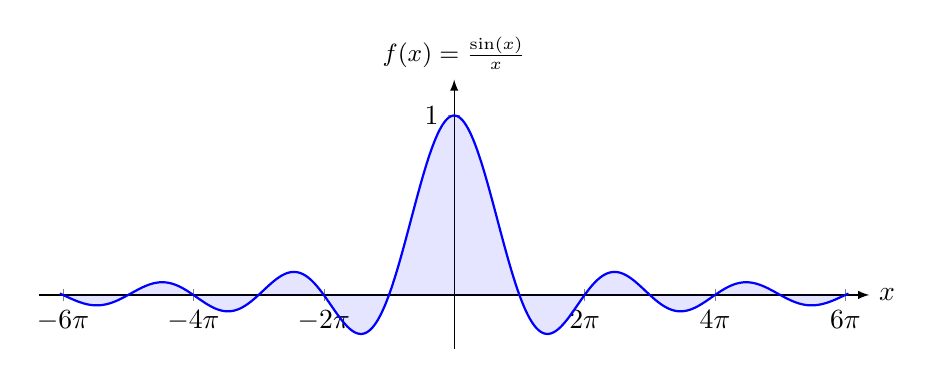
\begin{tikzpicture}
        \begin{axis}[
          axis lines = middle,
          xlabel = $x$,
          ylabel = {\small $f(x)=\frac{\sin(x)}{x}$},
          xmin = -20, xmax = 20,
          ymin = -0.3, ymax = 1.2,
          % Set x-ticks at multiples of pi
          xtick = {-6*pi, -4*pi, -2*pi, 0, 2*pi, 4*pi, 6*pi},
          xticklabels = {$-6\pi$, $-4\pi$, $-2\pi$, $0$, $2\pi$, $4\pi$, $6\pi$},
          ytick = {0, 1},
          samples = 500, % High sample count for smooth oscillations
          domain = -19:19,
          width = \linewidth, height = 5cm, % Changed width to fit minipage
          axis line style = {-latex}, % Arrows on axes
          % Adjust label positions
          every axis x label/.style={at={(ticklabel* cs:1.0)}, anchor=west},
          every axis y label/.style={at={(ticklabel* cs:1.0)}, anchor=south},
        ]
          % Plot sin(x)/x.
          \addplot [
            blue,
            thick,
            mark=none
          ] {x==0 ? 1 : sin(deg(x))/x};

          % Shading the area
          \addplot [
            fill=blue,
            fill opacity=0.1,
            draw=none,
          ] {x==0 ? 1 : sin(deg(x))/x} \closedcycle;

        \end{axis}
      \end{tikzpicture}
    \end{minipage}
    \hfill % Spacing between plots
    % ---- Right Plot: |f(x)| = |sin(x)/x| ----
    \begin{minipage}[b]{0.48\textwidth}
      \centering
      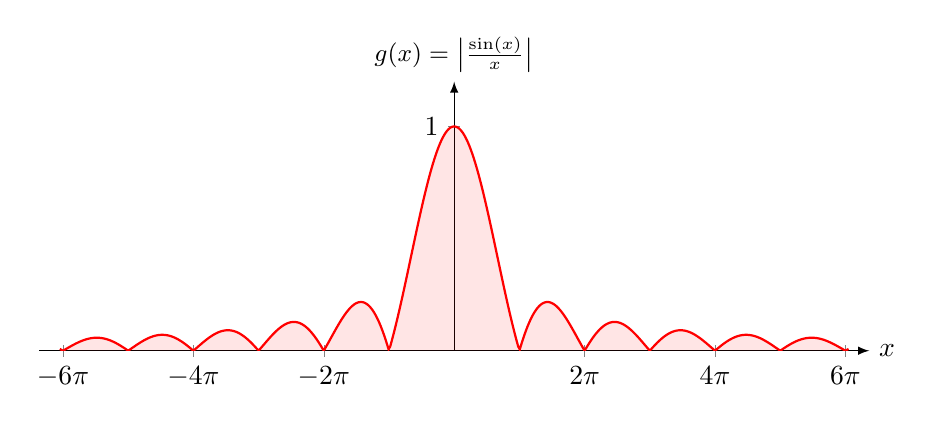
\begin{tikzpicture}
        \begin{axis}[
          axis lines = middle,
          xlabel = $x$,
          ylabel = {\small $g(x)=\left|\frac{\sin(x)}{x}\right|$}, % Updated Label
          xmin = -20, xmax = 20,
          ymin = 0, ymax = 1.2, % Updated ymin for absolute value
          % Set x-ticks at multiples of pi
          xtick = {-6*pi, -4*pi, -2*pi, 0, 2*pi, 4*pi, 6*pi},
          xticklabels = {$-6\pi$, $-4\pi$, $-2\pi$, $0$, $2\pi$, $4\pi$, $6\pi$},
          ytick = {0, 1},
          samples = 500,
          domain = -19:19,
          width = \linewidth, height = 5cm, % Width fits minipage
          axis line style = {-latex},
          % Adjust label positions
          every axis x label/.style={at={(ticklabel* cs:1.0)}, anchor=west},
          every axis y label/.style={at={(ticklabel* cs:1.0)}, anchor=south},
        ]
          % Plot abs(sin(x)/x).
          % Note the use of abs(...) around the expression
          \addplot [
            red, % Changed color to distinguish
            thick,
            mark=none
          ] {abs(x==0 ? 1 : sin(deg(x))/x)};

          % Shading the area under the absolute value curve
          \addplot [
            fill=red, % Changed fill color
            fill opacity=0.1,
            draw=none,
          ] {abs(x==0 ? 1 : sin(deg(x))/x)} \closedcycle;

        \end{axis}
      \end{tikzpicture}
    \end{minipage}

    \caption{In the example above, we can see $f(x) = \frac{\sin(x)}{x}$ converging due to the positive and negative parts canceling out, but the improper Riemann integral of $\big| \frac{\sin(x)}{x} \big|$ will diverge since it $f$ is not absolutely integrable. }
    \label{fig:sinc_comparison}
  \end{figure}

  It is important to see that the conditions for Riemann integrability is more strict, but Riemann integrability and the existence of the Riemann integral are pretty much equivalent. 
  \begin{equation}
    f \text{ (improperly) Riemann integrable} \iff \bigg| \int f \bigg| < +\infty
  \end{equation}
  However, we want to distinguish Lebesgue integrability and the existence of the Lebesgue integral. That is, only one direction holds, and a Lebesgue integral may exist even if a function is not Lebesgue integrable. 
  \begin{equation}
    f \text{ Lebesgue integrable} \iff \int |f| < +\infty \implies \bigg| \int f \bigg| < +\infty
  \end{equation}

  \begin{theorem}[Conditions of Lebesgue Integrability from Improper Riemann Integrability]
    If $f$ is improperly Riemann integrable over an interval $[a, \omega)$, and $\int |f| < +\infty$, then $f$ is Lebesgue integrable over $[a, \omega)$. 
  \end{theorem}
  \begin{proof}
    
  \end{proof}

  This following theorem on Riemmann integrability is much more restrictive, while for above, measurable functions can be very wild. 

  \begin{theorem}[Characterization of Riemann Integrability]
    $f$ is Riemann integrable on $[a, b]$ if the set of its discontinuities has measure $0$. 
  \end{theorem}
  \begin{proof}
    Not stated. In book. 
  \end{proof}

\subsection{Exercises} 

  \begin{exercise}[Royden 4.1]
    Show that, in the above Dirichlet function example, $\{f_n\}$ fails to converge to $f$ uniformly on $[0, 1]$.
  \end{exercise}

  \begin{exercise}[Royden 4.2]
    A partition $P^{\prime}$ of $[a, b]$ is called a refinement of a partition $P$ provided each partition point of $P$ is also a partition point of $P^{\prime}$. For a bounded function $f$ on $[a, b]$, show that under refinement lower Darboux sums increase and upper Darboux sums decrease.
  \end{exercise}

  \begin{exercise}[Royden 4.3]
    Use the preceding problem to show that for a bounded function on a closed, bounded interval, each lower Darboux sum is no greater than each upper Darboux sum. From this conclude that the lower Riemann integral is no greater than the upper Riemann integral.
  \end{exercise}

  \begin{exercise}[Royden 4.4]
    Suppose the bounded function $f$ on $[a, b]$ is Riemann integrable over $[a, b]$. Show that there is a sequence $\{P_n\}$ of partitions of $[a, b]$ for which $\lim_{n \to \infty} [U(f, P_n) - L(f, P_n)] = 0$.
  \end{exercise}

  \begin{exercise}[Royden 4.5]
    Let $f$ be a bounded function on $[a, b]$. Suppose there is a sequence $\{P_n\}$ of partitions of $[a, b]$ for which $\lim_{n \to \infty} [U(f, P_n) - L(f, P_n)] = 0$. Show that $f$ is Riemann integrable over $[a, b]$.
  \end{exercise}

  \begin{exercise}[Royden 4.6]
    Use the preceding problem to show that since a continuous function $f$ on a closed, bounded interval $[a, b]$ is uniformly continuous on $[a, b]$, it is Riemann integrable over $[a, b]$.
  \end{exercise}

  \begin{exercise}[Royden 4.7]
    Let $f$ be an increasing real-valued function on $[0, 1]$. For a natural number $n$, define $P_n$ to be the partition of $[0, 1]$ into $n$ subintervals of length $1/n$. Show that $U(f, P_n) - L(f, P_n) \leq 1/n[f(1) - f(0)]$. Use Problem 5 to show that $f$ is Riemann integrable over $[0, 1]$.
  \end{exercise}

  \begin{exercise}[Royden 4.8]
    Let $\{f_n\}$ be a sequence of bounded functions that converges uniformly to $f$ on the closed, bounded interval $[a, b]$. If each $f_n$ is Riemann integrable over $[a, b]$, show that $f$ also is Riemann integrable over $[a, b]$. Is it true that
    \begin{equation*}
      \lim_{n \to \infty} \int_a^b f_n = \int_a^b f \, ?
    \end{equation*}
  \end{exercise}

  \begin{exercise}[Royden 4.9][ex:royden4.9]
    Let $E$ have measure zero. Show that if $f$ is a bounded function on $E$, then $f$ is measurable and $\int_E f = 0$.
  \end{exercise}
  \begin{solution}
    For any measurable set $S$ in the codomain of $f$, 
    \begin{equation}
      m\big( f^{-1} (S) \big) \leq m(E) = 0 \implies f^{-1} (S) \text{ is measurable}
    \end{equation}
    Also, 
    \begin{equation}
      \int_E f \leq \int_E |f| \leq \int_E M = M \cdot m(E) = 0
    \end{equation}
  \end{solution}

  \begin{exercise}[Royden 4.10]
    Let $f$ be a bounded measurable function on a set of finite measure $E$. For a measurable subset $A$ of $E$, show that $\int_A f = \int_E f \cdot \chi_A$.
  \end{exercise}

  \begin{exercise}[Royden 4.11]
    Does the Bounded Convergence Theorem hold for the Riemann integral?
  \end{exercise}
  \begin{solution}
    No, look at sequence of functions pointwise converging to Dirichlet function on $[0, 1]$. They are uniformly bounded by $1$. 
  \end{solution}

  \begin{exercise}[Royden 4.12]
    Let $f$ be a bounded measurable function on a set of finite measure $E$. Assume $g$ is bounded and $f = g$ a.e. on $E$. Show that $\int_E f = \int_E g$.
  \end{exercise}
  \begin{solution}
    Let $f = g$ on $F \subset E$. Then, 
    \begin{align}
      \int_E f = \int_F f + \underbrace{\int_{E \setminus F} f}_{= 0} = \int_F f = \int_F g = \int_F g + \underbrace{\int_{E \setminus F} g}_{= 0} = \int_E g
    \end{align}
    where the labeled integrals equal $0$ from Exercise \ref{ex:royden4.9}. 
  \end{solution}

  \begin{exercise}[Royden 4.13]
    Does the Bounded Convergence Theorem hold if $m(E) < \infty$ but we drop the assumption that the sequence $\{|f_n|\}$ is uniformly bounded on $E$?
  \end{exercise}
  \begin{solution}
    No, consider the triangle function defined on $[0, 1/n]$ as $f(0) = 0$, $f(1/2n) = 2n$, $f(1/n) = 0$, and everything linearly interpolated. 
  \end{solution}

  \begin{exercise}[Royden 4.14]
    Show that Proposition 8 is a special case of the Bounded Convergence Theorem.
  \end{exercise}
  \begin{solution}
    It suffices to prove that $f_n \to f$ uniformly implies $f_n$ is uniformly bounded. $\forall \epsilon > 0$, $\exists N \in \mathbb{N}$ s.t. 
    \begin{equation}
      n \geq N \implies |f(x) - f_n (x)| < \epsilon \quad \forall x \in E
    \end{equation}
    So set $\epsilon > 1$ and then $N^\ast$ s.t. 
    \begin{equation}
      n \geq N^\ast |f - f_n| < 1 \implies |f_n| < |f| + 1
    \end{equation}
    So $f_n$ is uniformly bounded by $M_{N^\ast}$. The rest of the functions are bounded by $M_1, \ldots, M_{N^\ast - 1}$, so take the uniform bound 
    \begin{equation}
      M = \max \{M_1, \ldots, M_{N^\ast}\}
    \end{equation}
  \end{solution}

  \begin{exercise}[Royden 4.15]
    Verify the assertions in the last Remark of this section.
  \end{exercise}

  \begin{exercise}[Royden 4.16]
    Let $f$ be a nonnegative bounded measurable function on a set of finite measure $E$. Assume $\int_E f = 0$. Show that $f = 0$ a.e. on $E$.
  \end{exercise}
  \begin{solution}
    Assume $f \neq 0$ a.e. on $E$, so call this set $E_0 \subset E$. Then, 
    \begin{equation}
      \int_E f = \int_{E_0} f + \int_{E \setminus E_0} f \geq \int_{E_0} f
    \end{equation}
    Now we must prove $0 < \int_{E_0} f$. Define 
    \begin{equation}
      E_n = \{x \in E \colon f(x) > 1/n \} 
    \end{equation}
    Then, $E_n$ is ascending, and by continuity of measure from below, 
    \begin{equation}
      m(E_0) = m \bigg( \bigcup_n E_n \bigg) = \lim_{n \to \infty} m(E_n) 
    \end{equation}
    So $\forall \delta > 0$, we can choose $N \in \mathbb{N}$ s.t. 
    \begin{equation}
      m (E_0 \setminus E_N) < \delta, \quad f(x) > \frac{1}{N} \text{ on } E_N
    \end{equation}
    which implies 
    \begin{equation}
      \int_{E_0} f = \int_{E_N} f + \int_{E_0 \setminus E_N} f \geq \int_{E_N} f \geq \frac{1}{N} m(E_N) > \frac{1}{N} (m(E_0) - \delta) > 0
    \end{equation}
  \end{solution}

  \begin{exercise}[Royden 4.17]
    Let $E$ be a set of measure zero and define $f \equiv \infty$ on $E$. Show that $\int_E f = 0$.
  \end{exercise}
  \begin{solution}
    We know that 
    \begin{equation}
      \int_E f = \sup \bigg\{ \int_E \phi \colon \phi \leq h, \phi \text{ simple} \bigg\} 
    \end{equation}
    But for every $\phi$, it is simple and therefore bounded by $M_\phi$, and so 
    \begin{equation}
      \int_E \phi \leq \int_E M_\phi = M_\phi \cdot m(E) = 0
    \end{equation}
    So the supremum must be $0$. 
  \end{solution}

  \begin{exercise}[Royden 4.18]
    Show that the integral of a bounded measurable function of finite support is properly defined.
  \end{exercise}

  \begin{exercise}[Royden 4.19]
    For a number $\alpha$, define $f(x) = x^{\alpha}$ for $0 < x \leq 1$, and $f(0) = 0$. Compute $\int_0^1 f$.
  \end{exercise}

  \begin{exercise}[Royden 4.20]
    Let $\{f_n\}$ be a sequence of nonnegative measurable functions that converges to $f$ pointwise on $E$. Let $M \geq 0$ be such that $\int_E f_n \leq M$ for all $n$. Show that $\int_E f \leq M$. Verify that this property is equivalent to the statement of Fatou's Lemma.
  \end{exercise}

  \begin{exercise}[Royden 4.21]
    Let the function $f$ be nonnegative and integrable over $E$ and $\epsilon > 0$. 
    \begin{enumerate}
      \item Show there is a simple function $\eta$ on $E$ that has finite support, $0 \leq \eta \leq f$ on $E$ and $\int_E |f - \eta| < \epsilon$. 
      \item If $E$ is a closed, bounded interval, show there is a step function $h$ on $E$ that has finite support and $\int_E |f - h| < \epsilon$.
    \end{enumerate}
  \end{exercise}
  \begin{solution}
    Listed. 
    \begin{enumerate}
      \item $f \geq 0$ on $E$, integrable and so measurable. By SAT, $\exists$ increasing sequence of simply functions $\phi_n \to f$. By MCT, 
        \begin{equation}
          \lim_{n \to \infty} \int_E \phi_n = \int_E f
        \end{equation}
        So for $\epsilon > 0$, choose $N \in \mathbb{N}$ s.t. 
        \begin{equation}
          n \geq N \implies \bigg| \int_E f - \int_E \phi_n \bigg| < \epsilon
        \end{equation}
        Set $\eta = \phi_N$. Then, 
        \begin{equation}
          |f - \eta| = f - \eta \implies \bigg| \int_E f - \eta \bigg| = \int_E |f - \eta| < \epsilon 
        \end{equation}

      \item If $E$ is closed and bounded, then $\forall \delta > 0$, by Lusin's there exists continuous $g$ on closed set $F$ s.t. 
        \begin{equation}
          m(E \setminus F) \delta, \quad f = g \text{ on } F
        \end{equation}
        $f$ is continuous on $F$ and so it Riemann integrable $\implies \exists$ step function $\phi$ s.t. 
        \begin{equation}
          \bigg( \int_F f \bigg) - \frac{\epsilon}{2} < \int_F \phi < \int_F f
        \end{equation}
        By EVT, $f$ is bounded by $M$, so 
        \begin{equation}
          \int_{E \setminus F} |f| < M \cdot m(E \setminus F) \to 0
        \end{equation}
        So, set $\phi = 0$ on $E \setminus F$ and 
        \begin{equation}
          \int_E |f - \phi| = \underbrace{\int_F |f - \phi|}_{<\epsilon/2} + \underbrace{\int_{E \setminus F} |f|}_{< \epsilon/2} + \underbrace{\int_{E \setminus F} |\phi|}_{=0}
        \end{equation}
    \end{enumerate}
    \qed For the second part, I was thinking of Dini's. 
  \end{solution}

  \begin{exercise}[Royden 4.22]
    Let $\{f_n\}$ be a sequence of nonnegative measurable functions on $\mathbf{R}$ that converges pointwise on $\mathbf{R}$ to $f$ and $f$ be integrable over $\mathbf{R}$. Show that
    \begin{equation*}
      \text{if } \int_{\mathbf{R}} f = \lim_{n \to \infty} \int_{\mathbf{R}} f_n, \text{ then } \int_E f = \lim_{n \to \infty} \int_E f_n \text{ for any measurable set } E.
    \end{equation*}
  \end{exercise}

  \begin{exercise}[Royden 4.23]
    Let $\{a_n\}$ be a sequence of nonnegative real numbers. Define the function $f$ on $E = [1, \infty)$ by setting $f(x) = a_n$ if $n \leq x < n + 1$. Show that $\int_E f = \sum_{n=1}^{\infty} a_n$.
  \end{exercise}
  \begin{solution}
    Let $f_n = \sum_{k=1}^n a_k$. Then, $f_n$ is increasing, and $f_n \to f$. By MCT, 
    \begin{equation}
      \int_E f = \lim_{n \to \infty} \int_E f_n = \lim_{n \to \infty} \sum_{k=1}^n  a_k \cdot m([k, k +1)) = \sum_{k=1}^\infty a_k 
    \end{equation}
  \end{solution}

  \begin{exercise}[Royden 4.24]
    Let $f$ be a nonnegative measurable function on $E$.
    \begin{enumerate}
      \item Show there is an increasing sequence $\{\varphi_n\}$ of nonnegative simple functions on $E$, each of finite support, which converges pointwise on $E$ to $f$.
      \item Show that $\int_E f = \sup \{\int_E \varphi \mid \varphi \text{ simple, of finite support and } 0 \leq \varphi \leq f \text{ on } E\}$.
    \end{enumerate}
  \end{exercise}
  \begin{solution}
    Listed. 
    \begin{enumerate}
      \item By SAT, $\exists$ increasing sequence of $\phi_n$ simply on $E$ s.t. $\phi_n \to f$. Since $f \geq 0$, we can assume $\phi_n = 0$ if negative, which is still simple. For finite support, let's restrict each $\phi_n$ to be on $E_n = E \cap [-n, n]$, and let $\phi_n = 0$ elsewhere. This still preserves nonnegativity and $\phi_n \to f$. 
      \item By monotonicity, 
        \begin{equation}
          \forall n, \forall \phi_n \int_E f \geq \int_E \phi_n \implies \int_E f \geq \sup \int_E \phi
        \end{equation}
        By MCT, 
        \begin{equation}
          \int_E f = \lim_{n \to \infty} \int_E \phi_n = \lim_{n \to \infty} \sup_{k \geq n} \int_E \phi_k \leq \sup_n \int_E \phi_n
        \end{equation}
        where the final inequality follows from the limsup being a monotonically decreasing sequence as we are taking the supremum over a more restrictive class of functions.  
    \end{enumerate}
    \qed. Fatou is not a bad choice for 2, but we see that it leads nowhere since the inequality is in the wrong direction. 
    \begin{equation}
      \int_E f \leq \lim_{n \to \infty} \inf_{k \geq n} \int_E f_n \geq \inf_n \bigg\{ \int_E f_n \bigg\}
    \end{equation}
  \end{solution}

  \begin{exercise}[Royden 4.25]
    Let $\{f_n\}$ be a sequence of nonnegative measurable functions on $E$ that converges pointwise on $E$ to $f$. Suppose $f_n \leq f$ on $E$ for each $n$. Show that
    \begin{equation*}
      \lim_{n \to \infty} \int_E f_n = \int_E f.
    \end{equation*}
  \end{exercise}
  \begin{solution}
    By monotonicity, 
    \begin{equation}
      f \geq f_n \implies \int_E f \geq \int_E f_n \implies \int_E f \geq \limsup_n \int_E f_n
    \end{equation}
    By Fatou, 
    \begin{equation}
      \int_E f \leq \liminf_n \int_E f_n 
    \end{equation}
    By combining these inequalities we are done. 
  \end{solution}

  \begin{exercise}[Royden 4.26]
    Show that the Monotone Convergence Theorem may not hold for decreasing sequences of functions.
  \end{exercise}

  \begin{exercise}[Royden 4.27]
    Prove the following generalization of Fatou's Lemma: If $\{f_n\}$ is a sequence of nonnegative measurable functions on $E$, then
    \begin{equation*}
      \int_E \liminf f_n \leq \liminf \int_E f_n.
    \end{equation*}
  \end{exercise}
  \begin{solution}
    Let $g_n = \int_{k \geq n} f_k$ which is measurable and increasing. By MCT, 
    \begin{equation}
      \int_E \lim_{n \to \infty} \inf_{k \geq n} f_k = \int_E g = \lim_{n \to \infty} \int_E \inf_{k \geq n} f_k 
    \end{equation}
    But 
    \begin{align}
      \int_E \inf_{k \geq n} f_k & = \sup \bigg\{ \int h \colon h \text{ measurable, bounded, finite support}, h \leq \int_{k \geq n} f_k \bigg\} \\ 
                                 & = \inf_{k \geq n} \sup \bigg\{ \int h \colon h \text{ measurable, bounded, finite support}, h \leq f_k \bigg\} \\ 
                                 & = \inf_{k \geq n} \int_E f_k
    \end{align}
  \end{solution}

  \begin{exercise}[Royden 4.28]
    Let $f$ be integrable over $E$ and $C$ a measurable subset of $E$. Show that $\int_C f = \int_E f \cdot \chi_C$.
  \end{exercise}

  \begin{exercise}[Royden 4.29]
    For a measurable function $f$ on $[1, \infty)$ which is bounded on bounded sets, define $a_n = \int_n^{n+1} f$ for each natural number $n$. Is it true that $f$ is integrable over $[1, \infty)$ if and only if the series $\sum_{n=1}^{\infty} a_n$ converges? Is it true that $f$ is integrable over $[1, \infty)$ if and only if the series $\sum_{n=1}^{\infty} a_n$ converges absolutely?
  \end{exercise}

  \begin{exercise}[Royden 4.30]
    Let $g$ be a nonnegative integrable function over $E$ and suppose $\{f_n\}$ is a sequence of measurable functions on $E$ such that for each $n$, $|f_n| \leq g$ a.e. on $E$. Show that
    \begin{equation*}
      \int_E \liminf f_n \leq \liminf \int_E f_n \leq \limsup \int_E f_n \leq \int_E \limsup f_n.
    \end{equation*}
  \end{exercise}

  \begin{exercise}[Royden 4.31]
    Let $f$ be a measurable function on $E$ which can be expressed as $f = g + h$ on $E$, where $g$ is finite and integrable over $E$ and $h$ is nonnegative on $E$. Define $\int_E f = \int_E g + \int_E h$. Show that this is properly defined in the sense that it is independent of the particular choice of finite integrable function $g$ and nonnegative function $h$ whose sum is $f$.
  \end{exercise}

  \begin{exercise}[Royden 4.32]
    Prove the General Lebesgue Dominated Convergence Theorem by following the proof of the Lebesgue Dominated Convergence Theorem, but replacing the sequences $\{g - f_n\}$ and $\{g + f_n\}$, respectively, by $\{g_n - f_n\}$ and $\{g_n + f_n\}$.
  \end{exercise}
  \begin{solution}
    For all $n$, we have $|f_n| \leq g_n$ and $f_n \to f$, $g_n \to g$ a.e. on $E$. So, $|f| \leq g$ pointwise a.e. on $E$. Therefore, for all $n$ we have
    \begin{equation}
      |f_n - f| \leq g_n + g
    \end{equation}
    pointwise a.e. on $E$. Now apply Fatou to the nonnegative function $g_n + g - |f_n - f|$ to get 
    \begin{equation}
      \liminf_{n \to \infty} \int_E (g_n + g - |f_n - f|) \geq \int_E \liminf_{n \to \infty}(g_n + g - |f_n - f|) = 2 \int_E g
    \end{equation}
    The LHS equals 
    \begin{equation}
      \liminf_{n \to \infty} \int_E (g_n + g - |f_n - f|) = 2 \int_E g - \limsup_{n \to \infty} \int_E |f_n - f|
    \end{equation}
    since $\lim_{n \to \infty} \int_E g_n = \int_E g$. Substituting and applying the integral comparison test gives 
    \begin{equation}
      0 \geq \limsup_{n \to \infty} \left| \int_E (f_n - f) \right| \geq \liminf_{n \to \infty} \left| \int_E f_n - f \right| \geq 0 \implies \lim_{n \to \infty} \bigg| \int_E f_n - f \bigg| = 0  
    \end{equation}
    and by linearity, we can take the $\int_E f$ out. 
  \end{solution}

  \begin{exercise}[Royden 4.33]
    Let $\{f_n\}$ be a sequence of integrable functions on $E$ for which $f_n \to f$ a.e. on $E$ and $f$ is integrable over $E$. Show that $\int_E |f - f_n| \to 0$ if and only if $\lim_{n \to \infty} \int_E |f_n| = \int_E |f|$. (Hint: Use the General Lebesgue Dominated Convergence Theorem.)
  \end{exercise}
  \begin{solution}
    We prove bidirectionally. 
    \begin{enumerate}
      \item $(\rightarrow)$. $\forall \epsilon > 0$, $\exists N \in \mathbb{N}$ s.t. 
        \begin{align}
          n \geq N & \implies \int |f - f_n| < \epsilon \\ 
                   & \implies \epsilon \int |f - f_n| \geq \int | |f| - |f_n|| \geq \bigg| \int |f| - \int |f_n| \bigg| \\ 
                   & \implies \lim_{n \to \infty} \int_F |f_n| = \int |f| 
        \end{align}

      \item $(\leftarrow)$. Suppose $\lim_{n\to\infty} \int_E |f_n| = \int_E |f|$. Then, for all $n \in \mathbb{N}$,
      \begin{equation}
        \lim_{n\to\infty} \int_E (|f_n| + |f|) = 2\int_E |f| < \infty
      \end{equation}
      Since $|f_n - f| \leq |f_n| + |f|$ on $E$ for all $n$ and $|f - f_n| \to 0$ a.e. on $E$, we have
      \[
      \lim_{n\to\infty} \int_E |f - f_n| = 0
      \]
      by the general Lebesgue DCT. 
    \end{enumerate}
    \qed One wrong way I turned for the second part was that I use the wrong dominated bound $f_n \leq |f_n|$, so by GDCT, 
    \begin{equation}
      \lim_{n \to \infty} \int f_n = f
    \end{equation}
    But this doesn't lead anywhere. 
  \end{solution}

  \begin{exercise}[Royden 4.34]
    Let $f$ be a nonnegative measurable function on $\mathbf{R}$. Show that
    \begin{equation*}
      \lim_{n \to \infty} \int_{-n}^n f = \int_{\mathbf{R}} f.
    \end{equation*}
  \end{exercise}
  \begin{solution}
    We know 
    \begin{equation}
      \int_{-n}^n f = \int_{\mathbb{R}} \underbrace{f \cdot \chi_{[-n, n]}}_{f_n}
    \end{equation}
    See that $0 \leq f_n \leq f$, so by MCT, 
    \begin{equation}
      \int_{\mathbb{R}} f = \lim_{n \to \infty} \int_{\mathbb{R}} f_n = \lim_{n \to \infty} \int_{\mathbb{R}} f \cdot \chi_{[-n, n]} = \lim_{n \to \infty} \int_{-n}^n f
    \end{equation}
  \end{solution}

  \begin{exercise}[Royden 4.35]
    Let $f$ be a real-valued function of two variables $(x, y)$ that is defined on the square $Q = \{(x, y) \mid 0 \leq x \leq 1, 0 \leq y \leq 1\}$ and is a measurable function of $x$ for each fixed value of $y$. Suppose for each fixed value of $x$, $\lim_{y \to 0} f(x, y) = f(x)$ and that for all $y$, we have $|f(x, y)| \leq g(x)$, where $g$ is integrable over $[0, 1]$. Show that
    \begin{equation*}
      \lim_{y \to 0} \int_0^1 f(x, y) dx = \int_0^1 f(x) dx.
    \end{equation*}
    Also show that if the function $f(x, y)$ is continuous in $y$ for each $x$, then
    \begin{equation*}
      h(y) = \int_0^1 f(x, y) dx
    \end{equation*}
    is a continuous function of $y$.
  \end{exercise}

  \begin{exercise}[Royden 4.36]
    Let $f$ be a real-valued function of two variables $(x, y)$ that is defined on the square $Q = \{(x, y) \mid 0 < x < 1, 0 < y < 1\}$ and is a measurable function of $x$ for each fixed value of $y$. For each $(x, y) \in Q$ let the partial derivative $\partial f/\partial y$ exist. Suppose there is a function $g$ that is integrable over $[0, 1]$ and such that
    \begin{equation*}
      \left|\frac{\partial f}{\partial y}(x, y)\right| \leq g(x) \text{ for all } (x, y) \in Q.
    \end{equation*}
    Prove that
    \begin{equation*}
      \frac{d}{dy} \left[\int_0^1 f(x, y) dx\right] = \int_0^1 \frac{\partial f}{\partial y}(x, y) dx \text{ for all } y \in [0, 1].
    \end{equation*}
  \end{exercise}

  \begin{exercise}[Royden 4.37]
    Let $f$ be a integrable function on $E$. Show that for each $\epsilon > 0$, there is a natural number $N$ for which if $n \geq N$, then $\left|\int_{E_n} f\right| < \epsilon$ where $E_n = \{x \in E \mid |x| \geq n\}$.
  \end{exercise}
  \begin{solution}
    Since $f$ is integrable, $\int_E |f| < +\infty$. Note 
    \begin{equation}
      E_n = \{x \in E \colon |x| \geq n\}
    \end{equation}
    is decreasing, so by continuity of integrals, 
    \begin{equation}
      \lim_{n \to \infty} \int_{E_n} f = \int_{\cap_{n=1}^\infty E_n} f 
    \end{equation}
    But $\cap_{n=1}^\infty E_n = \emptyset$, so this term is $0$. By definition of the limit, $\forall \epsilon > 0$, $\exists N \in \mathbb{N}$ s.t. 
    \begin{equation}
      n \geq N \implies \bigg| \int_{E_n} f \bigg| < \epsilon
    \end{equation}
    \qed. Note that 
    \begin{enumerate}
      \item continuity of measure is not necessary here, since it is manifested by the continuity of the integral. 
      \item I was also thinking of using Chebyshev to bound the integral using the measure of $E_n$ which gets smaller, but writing out 
        \begin{equation}
          m(\{x \in E \colon |f(x)| \geq a \}) \leq \frac{1}{a} \int_E f 
        \end{equation}
        doesn't really lead anywhere since it is a lower bound on the integral. 
    \end{enumerate}
  \end{solution}

  \begin{exercise}[Royden 4.38]
    For each of the two functions $f$ on $[1, \infty)$ defined below, show that $\lim_{n \to \infty} \int_1^n f$ exists while $f$ is not integrable over $[1, \infty)$. Does this contradict the continuity of integration?
    \begin{enumerate}
      \item Define $f(x) = (-1)^n/n$, for $n \leq x < n + 1$.
      \item Define $f(x) = (\sin x)/x$ for $1 \leq x < \infty$.
    \end{enumerate}
  \end{exercise}

  \begin{exercise}[Royden 4.39]
    Prove the theorem regarding the continuity of integration.
  \end{exercise}

  \begin{exercise}[Royden 4.40]
    Let $f$ be integrable over $\mathbf{R}$. Show that the function $F$ defined by
    \begin{equation*}
      F(x) = \int_{-\infty}^x f \text{ for all } x \in \mathbf{R}
    \end{equation*}
    is properly defined and continuous. Is it necessarily Lipschitz?
  \end{exercise}

  \begin{exercise}[Royden 4.41]
    Show that Proposition 25 is false if $E = \mathbf{R}$.
  \end{exercise}

  \begin{exercise}[Royden 4.42]
    Show that Theorem 26 is false without the assumption that the $h_n$'s are nonnegative.
  \end{exercise}

  \begin{exercise}[Royden 4.43]
    Let the sequences of functions $\{h_n\}$ and $\{g_n\}$ be uniformly integrable over $E$. Show that for any $\alpha$ and $\beta$, the sequence of linear combinations $\{\alpha f_n + \beta g_n\}$ also is uniformly integrable over $E$.
  \end{exercise}

  \begin{exercise}[Royden 4.44]
    Let $f$ be integrable over $\mathbf{R}$ and $\epsilon > 0$. Establish the following three approximation properties.
    \begin{enumerate}
      \item There is a simple function $\eta$ on $\mathbf{R}$ which has finite support and $\int_{\mathbf{R}} |f - \eta| < \epsilon$ (Hint: First verify this if $f$ is nonnegative.]
      \item There is a step function $s$ on $\mathbf{R}$ which vanishes outside a closed, bounded interval and $\int_{\mathbf{R}} |f - s| < \epsilon$. (Hint: Apply part (i) and Problem 18 of Chapter 3.)
      \item There is a continuous function $g$ on $\mathbf{R}$ which vanishes outside a bounded set and $\int_{\mathbf{R}} |f - g| < \epsilon$.
    \end{enumerate}
  \end{exercise}

  \begin{exercise}[Royden 4.45]
    Let $f$ be integrable over $E$. Define $\hat{f}$ to be the extension of $f$ to all of $\mathbf{R}$ obtained by setting $\hat{f} \equiv 0$ outside of $E$. Show that $\hat{f}$ is integrable over $\mathbf{R}$ and $\int_E f = \int_{\mathbf{R}} \hat{f}$. Use this and part (i) and (iii) of the preceding problem to show that for $\epsilon > 0$, there is a simple function $\eta$ on $E$ and a continuous function $g$ on $E$ for which $\int_E |f - \eta| < \epsilon$ and $\int_E |f - g| < \epsilon$.
  \end{exercise}

  \begin{exercise}[Royden 4.46]
    (Riemann-Lebesgue) Let $f$ be integrable over $(-\infty, \infty)$. Show that
    \begin{equation*}
      \lim_{n \to \infty} \int_{-\infty}^{\infty} f(x) \cos nx \, dx = 0.
    \end{equation*}
    (Hint: First show this for $f$ is a step function that vanishes outside a closed, bounded interval and then use the approximation property (ii) of Problem 44.)
  \end{exercise}

  \begin{exercise}[Royden 4.47]
    Let $f$ be integrable over $(-\infty, \infty)$.
    \begin{enumerate}
      \item Show that for each $t$,
      \begin{equation*}
        \int_{-\infty}^{\infty} f(x) dx = \int_{-\infty}^{\infty} f(x + t) dx.
      \end{equation*}
      \item Let $g$ be a bounded measurable function on $\mathbf{R}$. Show that
      \begin{equation*}
        \lim_{t \to 0} \int_{-\infty}^{\infty} g(x) \cdot [f(x) - f(x + t)] = 0.
      \end{equation*}
    \end{enumerate}
    (Hint: First show this, using uniform continuity of $f$ on $\mathbf{R}$, if $f$ is continuous and vanishes outside a bounded set. Then use the approximation property (iii) of Problem 44.)
  \end{exercise}

  \begin{exercise}[Royden 4.48]
    Let $f$ be integrable over $E$ and $g$ be a bounded measurable function on $E$. Show that $f \cdot g$ is integrable over $E$.
  \end{exercise}

  \begin{exercise}[Royden 4.49]
    Let $f$ be integrable over $\mathbf{R}$. Show that the following four assertions are equivalent:
    \begin{enumerate}
      \item $f = 0$ a.e on $\mathbf{R}$.
      \item $\int_{\mathbf{R}} fg = 0$ for every bounded measurable function $g$ on $\mathbf{R}$.
      \item $\int_A f = 0$ for every measurable set $A$.
      \item $\int_O f = 0$ for every open set $O$.
    \end{enumerate}
  \end{exercise}

  \begin{exercise}[Royden 4.50]
    Let $\mathcal{F}$ be a family of functions, each of which is integrable over $E$. Show that $\mathcal{F}$ is uniformly integrable over $E$ if and only if for each $\epsilon > 0$, there is a $\delta > 0$ such that for each $f \in \mathcal{F}$,
    \begin{equation*}
      \text{if } A \subseteq E \text{ is measurable and } m(A) < \delta, \text{ then } \left|\int_A f\right| < \epsilon.
    \end{equation*}
  \end{exercise}

  \begin{exercise}[Royden 4.51]
    Let $\mathcal{F}$ be a family of functions, each of which is integrable over $E$. Show that $\mathcal{F}$ is uniformly integrable over $E$ if and only if for each $\epsilon > 0$, there is a $\delta > 0$ such that for all $f \in \mathcal{F}$,
    \begin{equation*}
      \text{if } U \text{ is open and } m(E \cap U) < \delta, \text{ then } \int_{E \cap U} |f| < \epsilon.
    \end{equation*}
  \end{exercise}

  \begin{exercise}[Royden 4.52]
    \begin{enumerate}
      \item Let $\mathcal{F}$ be the family of functions $f$ on $[0, 1]$, each of which is integrable over $[0, 1]$ and has $\int_0^1 |f| \leq 1$. Is $\mathcal{F}$ uniformly integrable over $[0, 1]$?
      \item Let $\mathcal{F}$ be the family of functions $f$ on $[0, 1]$, each of which is continuous on $[0, 1]$ and has $|f| \leq 1$ on $[0, 1]$. Is $\mathcal{F}$ uniformly integrable over $[0, 1]$?
      \item Let $\mathcal{F}$ be the family of functions $f$ on $[0, 1]$, each of which is integrable over $[0, 1]$ and has $\int_a^b |f| \leq b - a$ for all $[a, b] \subseteq [0, 1]$. Is $\mathcal{F}$ uniformly integrable over $[0, 1]$?
    \end{enumerate}
  \end{exercise}

  \begin{exercise}[Math 631 Fall 2025, Midterm Exercise 2]
    Compute
    \begin{equation}
      \lim_{n\rightarrow\infty}\int_{\mathbb{R}}\frac{n\sin(x/n)}{x(1+x^{2})}dx.
    \end{equation}
  \end{exercise}
  \begin{solution}
    Observe that
    \begin{equation}
      \lim_{n\rightarrow\infty}\frac{n}{x}\sin\frac{x}{n}=1
    \end{equation}
    for every $x \in \mathbb{R}$. Thus the limit above is equal to $1/(1+x^{2})$ for every $x$. Moreover,
    \begin{equation}
      \left|\frac{n}{x}\sin\frac{x}{n}\right|\le1
    \end{equation}
    for all $x, n$ since $|\sin y| \le |y|$ for all $y$. Therefore, if we denote $f_n(x) = \frac{n \sin(x/n)}{x(1+x^2)}$, then we have $f_n(x) \rightarrow f(x) \equiv 1/(1+x^2)$ pointwise as $n \rightarrow \infty$, and $|f_n(x)| \le f(x)$ for all $x, n$. But $f(x)$ is integrable. Recall that for a non-negative $f$,
    \begin{equation}
      \int_{\mathbb{R}} f dx = \sup_g \int g dx,
    \end{equation}
    where sup is taken over all bounded $g$ of finite support such that $0 \le g \le f$. We can take as test functions $f_R(x) = f(x)\chi_{[-R,R]}$ where $\chi_E$ denotes the characteristic function of the set $E$. Note that any test function $g \le f_R$ for large enough $R$. Letting $R \rightarrow \infty$, we find that
    \begin{align}
      \int f dx &= \lim_{R\rightarrow\infty} \int_{-R}^{R} f dx \\
      &= \tan^{-1}(R) - \tan^{-1}(-R) = \pi.
    \end{align}
  \end{solution}

  \begin{exercise}[Math 631 Fall 2025, Midterm Exercise 3]
    Is $\{x^\alpha\}_{-1 < \alpha < \infty}$ uniformly integrable on $[0, 1]$?
  \end{exercise}
  \begin{solution}
    No. Take $\epsilon = 1$. Suppose that there exists $\delta > 0$ such that if $m(E) < \delta$, then $\int_E |f| dx < 1$ for every $f$ in the given family. Note that
    \begin{equation}
      \int_{0}^{\delta/2} x^\alpha dx = \frac{1}{\alpha + 1}(\delta/2)^{\alpha+1}.
    \end{equation}
    Once $\delta$ is fixed, we can always find $\alpha$ close enough to $-1$ so that
    \begin{equation}
      \frac{1}{\alpha + 1}(\delta/2)^{\alpha+1} > 1.
    \end{equation}
    Contradiction.
  \end{solution}

  \begin{exercise}[Math 631 Fall 2025, Final Exam Exercise 5]
    Construct a function $f(x)\ge0$ that is finite a.e., but $f$ is not integrable on any subinterval of $[0, 1]$.
  \end{exercise}
  \begin{solution}
    Consider $g(x)=\sum_{k}2^{-k}|x-r_{k}|^{-1/2}$, where $r_{k}$ is a sequence enumerating all rational numbers in $[0, 1]$. Then
    \begin{equation}
      \|g\|_{L^{1}}\le2\sum_{k}2^{-k}<\infty,
    \end{equation}
    since each $|x-r_{k}|$ function is integrable and its $L^{1}$ norm over $[0, 1]$ does not exceed 2 by a simple estimate. Therefore, $g$ is finite a.e. Now take $f(x)=g(x)^{2}$. On one hand, clearly $f(x)$ is finite a.e. since $g$ is. On the other hand, for any $k$, we have
    \begin{equation}
      f(x)\ge2^{-2k}|x-r_{k}|^{-1}
    \end{equation}
    (simply ignore all other positive terms in the sum when squaring). This implies that $f$ is not integrable on any subinterval of $[0, 1]$.
  \end{solution}
